\documentclass[11pt,a4paper]{article}
\usepackage[T1]{fontenc}
\usepackage{lmodern}
\usepackage[a4paper,textwidth=163mm,top=22mm,bottom=24mm]{geometry}
\usepackage{amsmath,amssymb,graphicx,hyperref}
\usepackage{microtype,xcolor}
\usepackage[font=small,labelfont=bf]{caption}
\usepackage[section]{placeins}
\hypersetup{colorlinks=true,linkcolor=blue!45!black,urlcolor=blue!45!black,citecolor=blue!45!black}
\setlength{\emergencystretch}{2em}
\setlength{\parskip}{0.25em}
\renewcommand{\topfraction}{0.9}
\renewcommand{\textfraction}{0.08}
\renewcommand{\floatpagefraction}{0.75}
\title{Eigen: Choosing What a Computation Must Retain}
\hypersetup{pdftitle={Eigen: Choosing What a Computation Must Retain}}
\author{}
\date{}
\begin{document}
\begin{center}
{\Large\bfseries Eigen: Choosing What a Computation Must Retain\par}
\vspace{0.5em}
{\small Private manuscript candidate - independent review pending\par}
\end{center}
\vspace{0.4em}
\interfootnotelinepenalty=10000
\section{What must a computation retain?}
Eigen starts from a question about description: which distinctions must a computational system preserve to do useful work? A smaller representation is not necessarily a better one. It must still answer the question, predict the relevant change or reconstruct the information on which an action depends. We make that requirement explicit, account for its cost, and use the failure of an inadequate description to decide what to retain next.

Two tasks sharing one register provide a simple entry point. Sharing saves a resource, but the tasks may prefer different states. Their compromise has a price that further optimisation cannot remove. A summary of an evolving process faces a related choice: retain another variable, retain some history, or accept a specified prediction error. In a collection of records, the decisive distinction may be smaller still: whether a purchase preceded an approval. Keeping thousands of nearby passages is little help if the representation loses that relation.

The most useful evidence comes from constructions where we can see the choice change the answer. A conditional displacement absorbs a spin's coupling to its surrounding oscillators exactly, leaving a bounded correction from which its cold state can be predicted. A residual identifies a missing direction in a quantum trial space, and its excitation energy helps decide whether adding it is worthwhile. A compact continuation rule answers exact joint queries without scanning every record. These examples share a method: preserve the structure that makes the requested operation possible, then measure the cost of the remaining approximation.

A \emph{task} specifies the quantity to predict or operation to perform. A \emph{representation} is the object used in place of a more detailed description. Its \emph{retained distinctions} are the differences between situations that it can still express. A \emph{reconstruction} says what its smaller coordinates mean in the original space. A \emph{residual} measures the failure of a specified calculation to commute with that reduction. These definitions give compression a purpose. Total cost includes constructing, storing, updating and using the representation, together with recovering witnesses or correcting an inadequate answer.

Eigen's contribution is a proposed synthesis and a method of construction, developed across mathematical papers, finite computational prototypes and a working research environment. Familiar objects - probability distributions, projections, effective operators and dependency graphs - acquire particular jobs within that method. The claim is strongest where the maps, assumptions and comparison can be written down. The larger proposition is that treating representation choice as part of the calculation can expose useful structure that a single global description obscures.

The article follows that proposition through three questions. First, when does an additional distinction earn its cost? The shared-register example leads to predictive loss, coarse dynamics and effective physical laws. Second, how does the account change a practical procedure? Quantum trial-space repair, spectral filtering and Dynamic Memory provide distinct answers. Third, how can the resulting knowledge remain usable when its sources or assumptions change? The Writing App retains scientific objects, their grounds and authorised transitions, providing an implemented counterpart and a route towards an extensible software development kit (SDK).

The evidence has different strengths at these three levels. Finite mathematical identities explain mechanisms. Simulations and archived comparisons establish particular outcomes under stated conditions. The software demonstrates persistent objects and recoverable operations. The SDK describes a product direction to evaluate. We develop each at the point where it advances the argument, so the reader can judge both the present contribution and the next useful test.

\section{The price of a new distinction}
\label{section:the-price-of-a-shared-description}

Suppose two computations use the same stored parameter $q\in\mathbb R^2$. One prefers $a=(1,0)$ and the other prefers $b=(\cos\theta,\sin\theta)$. Their losses are
\begin{equation}
 \ell_1(q)=\tfrac12\|q-a\|^2,\qquad
 \ell_2(q)=\tfrac12\|q-b\|^2,\qquad
 d^2=\|a-b\|^2=2(1-\cos\theta).
 \label{eq:register-losses}
\end{equation}
We take $0\leq\theta\leq\pi$. Here $\theta$ measures disagreement between the tasks and $d$ is the distance between their preferred settings. Neither task is difficult on its own. The difficulty comes from asking one register to serve both.

Give the first task weight $\alpha$ and the second weight $1-\alpha$, with $0\leq\alpha\leq1$. Completing the square gives
\begin{equation}
 \alpha\ell_1+(1-\alpha)\ell_2
 =\tfrac12\|q-q_*\|^2+\tfrac12\alpha(1-\alpha)d^2,
 \qquad q_*=\alpha a+(1-\alpha)b.
 \label{eq:register-square}
\end{equation}
The first term can be removed by optimisation. The second cannot: it is the price of the compromise within this representation. At equal weights it is $d^2/8$. If maintaining a second register costs an additional $c$, separate descriptions are preferable when $c<d^2/8$. The relevant comparison is between the total costs of two ways of performing the same pair of tasks, not between their storage sizes in isolation.

\emph{Self-Consistent Loss Geometries}~\cite{McCaulda239a} develops a coupled-evaluator model in which the system can also change the attention paid to each task. It adds a conflict charge $\gamma\alpha(1-\alpha)d^2$ and an arbitration penalty $2\eta(\alpha-\tfrac12)^2$. The parameters $\gamma\geq0$ and $\eta>0$ specify those modelled costs. The second penalty makes ignoring a task costly. After optimising $q$ and $\alpha$, the fixed shared-register model has
\begin{equation}
 L_B^*=\min\left\{\frac{d^2}{4}\left(\tfrac12+\gamma\right),
                         \frac{\eta}{2}\right\}.
 \label{eq:shared-optimum}
\end{equation}
Its options are balanced compromise or suppression of one evaluator. In the split option each task has its own minimising coordinate, removing the disagreement penalty by construction. The remaining incremental partition cost is $C_{\rm part}\geq0$, so the system achieves
\begin{equation}
 L_C^*=\min\{L_B^*,C_{\rm part}\}.
 \label{eq:partition-optimum}
\end{equation}
Figure~\ref{fig:dd-shared-register-price} makes the choice visible. At the stated register price, splitting becomes favourable before the fixed shared representation would suppress an evaluator. The useful adaptation is a change in what the register distinguishes.
\begin{figure}[htbp]
\centering
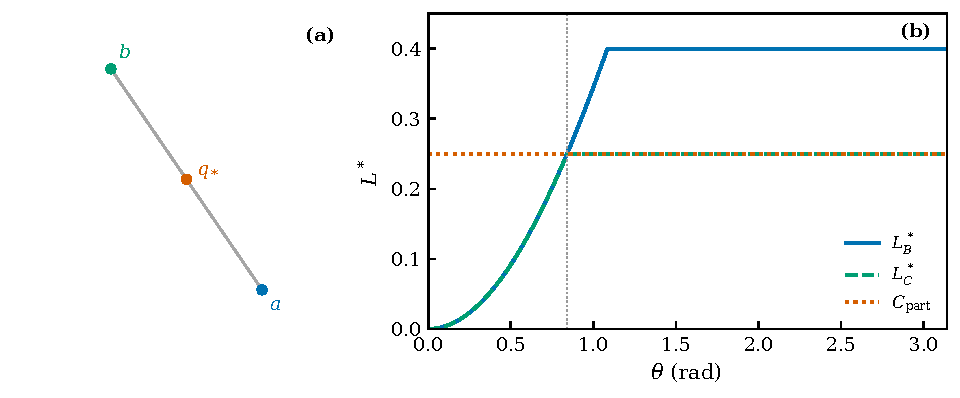
\includegraphics[width=\linewidth]{figures/portable-run-b69220b3a27348ad.result/dd-shared-register-price.pdf}
\caption{When should two tasks stop sharing a register? (a) The equally weighted quadratic compromise is $q_*=(a+b)/2$. (b) Fixed-register loss $L_B^*$ and partition-enabled loss $L_C^*$ versus disagreement angle $\theta$, for $\gamma=1$, $\eta=0.8$ and $C_{\rm part}=0.25$. Splitting becomes cheaper at $\theta=0.8411$ radians, before the fixed-register model suppresses an evaluator at $1.0853$. The curves evaluate the classical cost model in Eqs.~\eqref{eq:shared-optimum}--\eqref{eq:partition-optimum}.}
\label{fig:dd-shared-register-price}
\end{figure}

The classical model turns representation choice into an ordinary optimisation: tolerate the compromise or pay to remove it. The same question will recur in the quantum and memory examples: when should additional capacity buy a new distinction rather than more work inside the existing description?
\subsection{When a second register is worth its price}
Varying the register price as well as the disagreement reveals three regimes, shown in Figure~\ref{fig:dd-register-phase-diagram}. The boundary follows directly from the same objective. Write $A(\theta)=(\tfrac12+\gamma)d^2$. After minimising the shared coordinate, its remaining attention cost is
\[
 \frac{A(\theta)}4+\bigl(2\eta-A(\theta)\bigr)
                   \left(\alpha-\tfrac12\right)^2.
\]
Balanced sharing is therefore optimal when $A<2\eta$, while the shared model suppresses one evaluator when $A>2\eta$. Allowing the register itself to split gives the short result
\begin{equation}
 L_*=\min\left\{C_{\rm part},\frac{A(\theta)}4,\frac{\eta}2\right\},
 \qquad
 C_{\rm crit}(\theta)=
 \min\left\{\frac{\tfrac12+\gamma}{2}(1-\cos\theta),\frac{\eta}2\right\}.
 \label{eq:register-phase-boundary}
\end{equation}
For $C_{\rm part}<C_{\rm crit}$, two registers are preferable. Above the boundary, one is cheaper. Equality gives tied representations. The optimal cost is continuous across the share--split boundary, but generically has a kink as the preferred number of registers changes. This is an optimisation phase transition in a finite model.

At $A=2\eta$, every shared attention weight is degenerate. This boundary is reachable for $0\leq\theta\leq\pi$ when $\eta\leq2(\tfrac12+\gamma)$. The flat part of the boundary is informative. Once conflict is sufficiently large, the shared model can pay $\eta/2$ to abandon an evaluator instead of buying a second register. With $\gamma=1$ and $\eta=0.8$, the three regions meet at $\theta_{\rm att}=\arccos(1-\eta/(\tfrac12+\gamma))\simeq1.0853$ and $C_{\rm part}=0.4$. The earlier $C_{\rm part}=0.25$ example is a horizontal slice: increasing disagreement crosses from balanced sharing to separate registers at $\theta_{\rm split}\simeq0.8411$. The diagram makes the design choice explicit - tolerate a compromise, pay for another distinction, or sacrifice one of the tasks.

\begin{figure}[htbp]
\centering
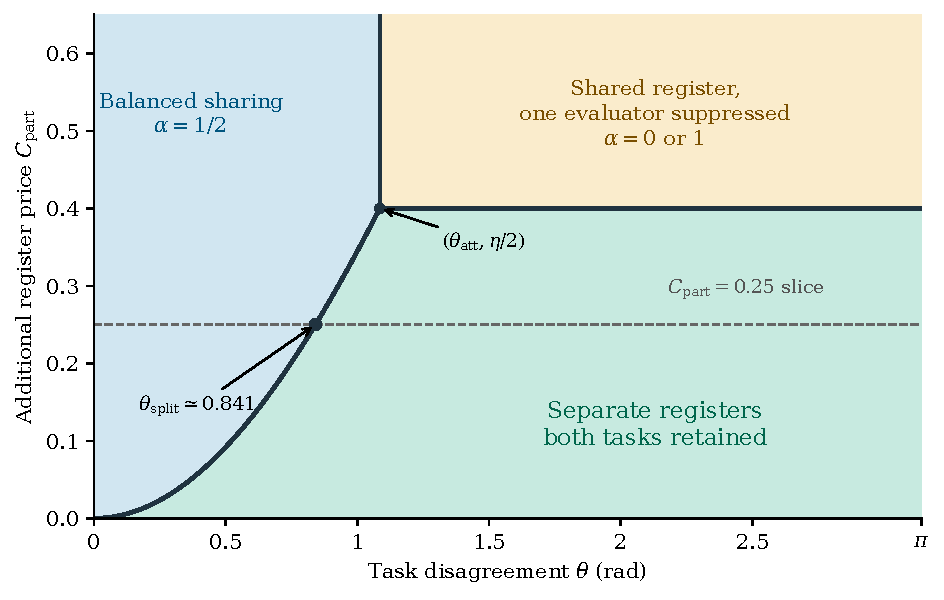
\includegraphics[width=0.93\linewidth]{figures/phase-run-939b6a8b76724d02.result/dd-register-phase-diagram.pdf}
\caption{The register-choice phase diagram for $\gamma=1$ and $\eta=0.8$. Below $C_{\rm crit}(\theta)$, splitting retains both tasks. Above it, the shared optimum is balanced at small $\theta$ and suppresses an evaluator at large $\theta$. Solid boundaries mark tied costs, including the vertical attention boundary above the meeting point. At that meeting point all shared attention weights are degenerate and splitting has the same cost. The dashed $C_{\rm part}=0.25$ slice recovers Figure~\ref{fig:dd-shared-register-price}. The regions are the exact optima of the declared finite model.}
\label{fig:dd-register-phase-diagram}
\end{figure}

\subsection{A cost coordinate and a task}\label{subsec:cost-task}
The register example assumes a price for an extra description. A separate question is how to choose a cost coordinate when independent capacities compose. \emph{The Cost of Complexity} and \emph{Foundations of Synthetics} motivate a logarithmic coordinate from multiplicative capacity and additive cost.~\cite{Reference975536} If independent capacities $M$ and $N$ compose multiplicatively, while their costs add, a nondecreasing cost function obeying $f(MN)=f(M)+f(N)$ has the form $f(N)=\kappa\log N$. The scale $\kappa\geq0$ fixes the cost unit. The premise concerns the capacity or product-order count being composed. A single globally sorted probability rank is a different object and need not multiply. This distinction matters: forcing two partially ordered descriptions into one global list can introduce comparisons that neither task required.

For fixed labels $r=1,\ldots,R$ with cost $\log r$, maximum entropy chooses the least concentrated probability law compatible with a specified mean cost. The partition sum below normalises those probabilities. The resulting family is
\begin{equation}
 p_\lambda(r)=\frac{r^{-\lambda}}{Z_R(\lambda)},\qquad
 Z_R(\lambda)=\sum_{r=1}^{R}r^{-\lambda}.
 \label{eq:cost-family}
\end{equation}
The multiplier $\lambda$ is the price conjugate to mean log-cost. Increasing it concentrates probability on cheaper labels. If $C_R=\sum_r p_\lambda(r)\log r$, then
\begin{equation}
 C_R=-\partial_\lambda\log Z_R,\qquad
 -\frac{dC_R}{d\lambda}
 =\operatorname{Var}_{p_\lambda}(\log r)
 =g_{\lambda\lambda}.
 \label{eq:cost-geometry}
\end{equation}
The response coefficient measures how distinguishable nearby probability laws are. It is also the Fisher information of this same one-parameter family, obtained by averaging $(\partial_\lambda\log p_\lambda)^2$. Thus cost response and statistical distinguishability are two readings of one construction. For a small change $\delta\lambda$, the relative entropy is
$D(p_\lambda\|p_{\lambda+\delta\lambda})
=\tfrac12g_{\lambda\lambda}(\delta\lambda)^2+O((\delta\lambda)^3)$.
This is a specific bridge from a cost coordinate to geometry, with the underlying probability distribution held in view. Calibrating $C_{\rm part}$ in seconds, joules or bytes is a further application-level task: the representational price must be connected to the resources and prediction error that matter.

At finite $R$ these expressions are smooth. The infinite counting-measure model has $Z_\infty(\lambda)=\zeta(\lambda)$ only for $\lambda>1$, and becomes singular at its normalisability boundary. This distinguishes a singular infinite limit from the smooth finite models. Physical heat, in turn, is charged to an operation on an ensemble. Landauer's reset analysis concerns the effect of a specified erasure protocol on information-bearing physical states.\footnote{R. Landauer, \emph{Irreversibility and Heat Generation in the Computing Process}, IBM Journal of Research and Development 5 (1961), \href{https://doi.org/10.1147/rd.53.0183}{doi:10.1147/rd.53.0183}.} Foundations makes this distinction concrete using retained side information and explicit bath/register operations.~\cite{Landauer1961f2ecf4}

A task supplies the other half of the accounting. Let $\Omega$ denote the underlying situation, $X$ its retained description and $Y$ the quantity to be predicted. For an encoder with $Y$ conditionally independent of $X$ given $\Omega$, and a decoder distribution $q(Y|X)$, the expected logarithmic prediction loss separates as
\begin{equation}
 \mathbb E[-\log q(Y|X)]
 =H(Y|\Omega)+I(Y;\Omega|X)
   +\mathbb E_X D\!\left(P(Y|X)\|q(Y|X)\right).
 \label{eq:predictive-loss}
\end{equation}
Here $H$ is the uncertainty left after the stated condition is known. The conditional mutual information $I(Y;\Omega|X)$ measures the predictive information about $Y$ available in $\Omega$ but absent from $X$. Relative entropy is $D(p\Vert q)=\sum_y p(y)\log[p(y)/q(y)]$: the excess expected logarithmic prediction loss from using $q$ when the outcomes follow $p$. The three terms are the target's intrinsic uncertainty, the predictive information lost by the encoder, and the decoder's mismatch. Better decoding cannot recover a distinction that was discarded. A larger description cannot remove randomness already present in the target.

Foundations illustrates this with three input bits $(a,b,c)$. The bit $c$ labels a sensor but does not affect the alarm probability. For $(a,b)=(00,01,10,11)$ those probabilities are $0.1,0.3,0.7,0.9$. Retaining $(a,b)$ preserves the forecasts exactly while discarding $c$. Retaining only $a$ gives the coarser forecasts $0.2$ and $0.8$ under the declared uniform input law. The adequate representation depends on the prediction being requested, not on preserving every input bit.

The next distinction can also have a local value. With a false stop costing one unit and a missed alarm three, the optimal alarm threshold is probability $1/4$. After observing $a=0$, acquiring $b$ reduces conditional decision risk from $0.6$ to $0.5$. After $a=1$, it does not change the preferred action. At acquisition cost $k<0.1$, buying $b$ only on the first branch improves total expected cost from $0.40$ to $0.35+0.5k$. Uniformly increasing resolution would pay for information where it changes nothing.

This also explains why a purely greedy refinement rule can be inadequate. A local step may cost more than its immediate benefit but unlock a valuable later calculation. For a finite refinement tree, an incremental gain $a_v$ at node $v$ and conditional child probabilities $q(u|v)$ give the backward recursion
\begin{equation}
 V(v)=\max\left\{0,\ a_v+\sum_u q(u|v)V(u)\right\}.
 \label{eq:refinement-value}
\end{equation}
A step with immediate gain $-1$ can be worthwhile if it unlocks gain $5$ with probability $0.6$: its continuation value is $2$. Efficient representation is a policy for purchasing the distinctions and intermediate constructions that make useful work possible. When the task is to predict an evolving process, the value of a distinction depends on what it lets us say about the future. A summary that answers today's question may not contain enough information to answer tomorrow's.


\section{What a summary must remember}
\label{section:what-a-useful-summary-must-remember}

Imagine a process that moves among four states. States 1 and 2 belong to region A, and states 3 and 4 to region B. Motion within either region is fast. There are also two routes between the regions, one slow and one three times faster. A reader interested only in the probability of being in A might reasonably try to replace the four states by two.

That summary loses something immediately. Starting in state 1 or state 2 gives the same retained probability, $p_A(0)=1$, but different initial escape rates: $p_A'(0)=-1$ or $-3$ in the chosen time units. No autonomous two-state law can assign both derivatives to the same initial state. Figure~\ref{fig:dd-retention-memory} shows the missing distinction and two ways to retain its effect.
\begin{figure}[htbp]
\centering
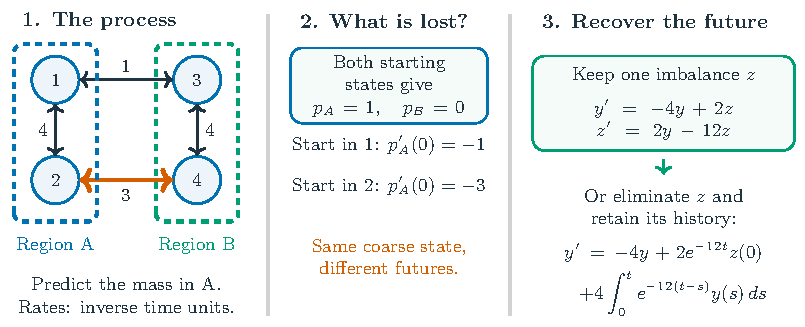
\includegraphics[width=\linewidth]{figures/portable-run-b69220b3a27348ad.result/dd-retention-memory.pdf}
\caption{What the coarse state omits. Four states exchange probability at the labelled symmetric rates. Starting in state 1 or 2 gives $p_A(0)=1$, but initial rates $-1$ and $-3$. Retaining $z=(p_1-p_2)-(p_3-p_4)$ closes the prediction for $y=p_A-p_B$, with $\dot y=-4y+2z$ and $\dot z=2y-12z$. Eliminating $z$ gives an exact memory term instead. This constructed example makes the retention and residual mechanisms explicit.}
\label{fig:dd-retention-memory}
\end{figure}

The example uses a column probability vector $p=(p_1,p_2,p_3,p_4)^T$ and the generator
\begin{equation}
 \dot p=Gp,\qquad
 G=\begin{pmatrix}
 -5&4&1&0\\
 4&-7&0&3\\
 1&0&-5&4\\
 0&3&4&-7
 \end{pmatrix},\qquad
 C=\begin{pmatrix}1&1&0&0\\0&0&1&1\end{pmatrix}.
 \label{eq:four-state}
\end{equation}
Off-diagonal entries of $G$ are transition rates and each column sums to zero, preserving total probability. The rectangular matrix $C$ retains $(p_A,p_B)^T=Cp$. It is an explicitly many-to-one map between two spaces of probability distributions.

A reconstruction map specifies what the reduced description stands for. Given a strictly positive reference distribution $\pi$, the conditional reconstruction associated with this partition is
\begin{equation}
 R=D_\pi C^T D_{C\pi}^{-1},\qquad CR=I,\qquad B=CGR,
 \label{eq:reconstruction}
\end{equation}
where $D_v$ is the diagonal matrix with vector $v$ on its diagonal. Within each coarse cell, $R$ restores the relative weights supplied by $\pi$. Here the stationary distribution is uniform, so $R=C^T/2$ and
$B=\left(\begin{smallmatrix}-2&2\\2&-2\end{smallmatrix}\right)$.
The reduced law predicts the average escape rate, not either hidden starting state separately.

The discrepancy between evolving first and reducing first is the closure residual
\begin{equation}
 \Delta=CG-BC.
 \label{eq:closure-residual}
\end{equation}
It maps a fine distribution to the difference between two proposed coarse derivatives. If $\Delta=0$, the retained state evolves autonomously for every fine initial distribution. For a partition of a Markov chain, this requires all fine states in a coarse cell to have the same total exit rate into each other coarse cell. The usual name is strong lumpability. Matching an equilibrium distribution is much weaker: with the stationary fit in Eq.~\eqref{eq:reconstruction}, $\Delta\pi=0$ even when the other states do not close.

The residual has a quantitative use beyond detecting exact failure. For finite Markov generators,
\begin{equation}
 C e^{tG}-e^{tB}C
 =\int_0^t e^{(t-s)B}\Delta e^{sG}\,ds.
 \label{eq:duhamel}
\end{equation}
Because stochastic evolution contracts the $\ell^1$ norm, a probability vector satisfies
$\|(C e^{tG}-e^{tB}C)p\|_1\leq\min\{2,t\|\Delta\|_1\}$.
Here $\|\Delta\|_1$ is the induced matrix $1$-norm. The horizon $t$ matters. A small instantaneous discrepancy may accumulate, and a bound useful for a short prediction need not justify indefinitely reusing the same reduced law.

For the four-state process, a particularly economical repair is to retain one imbalance,
\[
 y=p_1+p_2-p_3-p_4,\qquad
 z=p_1-p_2-p_3+p_4.
\]
Direct multiplication of Eq.~\eqref{eq:four-state} gives
\begin{equation}
 \dot y=-4y+2z,\qquad \dot z=2y-12z.
 \label{eq:two-coordinate}
\end{equation}
These two coordinates close exactly for the desired task, predicting $p_A=(1+y)/2$ while leaving other microstate distinctions unresolved.

Alternatively, solve the second equation for $z$ and substitute it into the first:
\begin{equation}
 \dot y(t)=-4y(t)+2e^{-12t}z(0)
       +4\int_0^t e^{-12(t-s)}y(s)\,ds.
 \label{eq:four-state-memory}
\end{equation}
The extra variable has become a memory kernel and an initial-condition term. The discarded coordinate's influence is retained through the history. Figure~\ref{fig:dd-retention-trajectories} compares the exact trajectories with the two-state approximation that omits this information.
\begin{figure}[htbp]
\centering
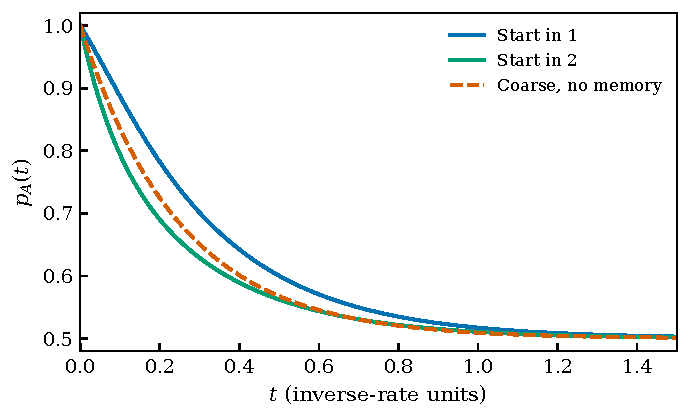
\includegraphics[width=\linewidth]{figures/portable-run-b69220b3a27348ad.result/dd-retention-trajectories.pdf}
\caption{Equal summaries, different futures. Exact region probabilities $p_A(t)$ for the four-state process, starting in state 1 or 2. The coarse model without the hidden imbalance $z$ predicts the same curve for both initial states. It initially lies between the exact trajectories but does not remain between them. Retaining $z$, or its exact memory kernel, recovers both trajectories. Time $t$ is in inverse base-rate units. The curves are analytic trajectories of Eq.~\eqref{eq:four-state}.}
\label{fig:dd-retention-trajectories}
\end{figure}

This is the elementary form of an established projection method. For a linear evolution $\dot x=Lx$, a projection $P$ and $Q=I-P$, write $u=Px$ and $w=Qx$. Exact elimination of $w$ gives
\begin{align}
 \dot u(t)={}&PLP\,u(t)+PLQ\,e^{tQLQ}w(0)\nonumber\\
 &+\int_0^t PLQ\,e^{(t-s)QLQ}QLP\,u(s)\,ds.
 \label{eq:general-memory}
\end{align}
Mori's original treatment makes clear why choosing the retained variables is decisive: a slow mode left in the discarded sector can invalidate a supposed short-memory approximation.\footnote{H. Mori, \emph{Transport, Collective Motion, and Brownian Motion}, Progress of Theoretical Physics 33 (1965),423--455, \href{https://doi.org/10.1143/ptp.33.423}{doi:10.1143/ptp.33.423}.} A local-in-time replacement needs a separation of scales or another explicit error control. Elimination alone supplies neither dissipation nor thermalisation.~\cite{Mori19656369be}

Hierarchy becomes useful when these accounts compose. If $C_{01}$ reduces level 0 to level 1 and $C_{12}$ reduces level 1 to level 2, their defects obey
\begin{equation}
 \Delta_{02}=C_{12}\Delta_{01}+\Delta_{12}C_{01}.
 \label{eq:composed-residual}
\end{equation}
The coarse model inherits the earlier mismatch as well as adding its own. A parent cannot declare itself accurate merely because it fits the already truncated child. This is the mathematical reason to transport an error account with a retained object.

Closure must still serve a task. Foundations enumerates all 2,047 bipartitions of a twelve-state model with three motifs. Its exactly closed hub/spoke partition retains essentially none of the motif-label information the task asks for. Imposing a retention requirement instead exposes a useful trade-off between predictive closure and the distinctions being preserved. The source also finds that an appropriate sign cut of the slow eigenfunction selects a good partition. The task determines which spectral or closure criterion is useful.

Each repair preserves fidelity under a specified operation. A useful summary preserves a forecast or decision. A useful reduced dynamical state carries enough information to predict its evolution. A useful hierarchy carries the inherited cost of what it discarded. These requirements give the next representation a job, rather than treating increasing abstraction as an achievement in itself.


\section{Effective laws after eliminating variables}
\label{section:loss-dynamics-and-the-choice-of-scale}

To decide which distinctions are worth retaining, we also need to say what counts as an error. A loss function says which answers we prefer. It does not yet say how a system moves between them. The distinction matters because two procedures can have the same optimum and radically different routes towards it. A probability distribution over possible configurations gives one way to describe both uncertainty and exploration. Relative entropy then prices departure from a reference distribution, while a generator specifies the actual motion.

The Law of Laws develops this combination in the functional
\begin{equation}
 {\cal F}[p]=\sum_x p(x)K(x)+M\sum_x p(x)\log\frac{p(x)}{q(x)},
 \qquad
 p_*(x)=\frac{q(x)e^{-K(x)/M}}{Z}.
 \label{eq:law-functional}
\end{equation}
Here $p$ is a normalised distribution, $q$ a positive normalised reference, $K$ the cost of a configuration and $M>0$ the price of concentrating probability away from $q$. The normalising constant is $Z=\sum_xq(x)e^{-K(x)/M}$. Substitution gives the exact identity
\[
 {\cal F}[p]-{\cal F}[p_*]=M D_{\rm KL}(p\Vert p_*),
 \qquad {\cal F}[p_*]=-M\log Z.
\]
The preferred distribution is therefore fixed by an explicit competition between cost and concentration.~\cite{Reference0e02fc} The relative entropy on the right measures the excess objective.

This construction survives elimination of hidden variables in a useful sense. Write the configuration as $(y,\xi)$, with retained coordinate $y$ and discarded coordinate $\xi$. Summing over $\xi$ gives the effective cost
\begin{equation}
 K_{\rm eff}(y)
 =-M\log\sum_\xi q(\xi|y)e^{-K(y,\xi)/M}.
 \label{eq:effective-law}
\end{equation}
The marginal distribution has the same form as Eq.~\eqref{eq:law-functional}, now with reference $q(y)$ and cost $K_{\rm eff}(y)$. A description can remain in one mathematical family while its parameters change with resolution. For the source's elementary Ising example, each spin is a sign $\sigma_i=\pm1$ and a neighbouring pair has energy $-J\sigma_i\sigma_{i+1}$. Eliminating a middle spin means summing its two possible signs. For retained neighbours $a,c=\pm1$, the factor is $\sum_{u=\pm1}e^{Ju(a+c)/M}=2\cosh[J(a+c)/M]$. Matching the factors for $a=c$ and $a=-c$ changes the nearest-neighbour coupling to $J'=(M/2)\log\cosh(2J/M)$. The coordinate $x=\tanh(J/M)$ obeys the simple map $x'=x^2$. This is a concrete instance of the renormalisation idea: follow how an effective description changes, rather than insisting that its original parameters survive intact.

A stationary distribution does not specify a clock. Different generators can preserve the same distribution, and non-reversible ones can circulate probability around it. The equilibrium elimination in Eq.~\eqref{eq:effective-law} consequently does not establish the dynamical closure in Eq.~\eqref{eq:closure-residual}. The two results complement one another. One constructs an effective cost. The other tests whether the chosen retained state has enough information to evolve autonomously.

\subsection{A subsystem retains its surroundings' influence}
Eliminating variables becomes a physical question when they describe an interacting environment. A qubit in a device is not an isolated two-state object. It interacts with nearby modes, control circuitry and other degrees of freedom. Those interactions can change both its equilibrium probabilities and the information needed to predict its motion. Drawing a boundary around the qubit does not switch the interactions off. It changes what we must encode on the inside if we no longer describe the outside explicitly. A qubit has two basis states. We write a state column vector as $|\psi\rangle$ and its conjugate transpose as $\langle\psi|$, so $\langle\psi|O|\psi\rangle$ is ordinary matrix multiplication giving the mean measured value of an observable $O$. Observables are represented by Hermitian matrices, equal to their conjugate transpose and with real eigenvalues. The energy observable is called the Hamiltonian.

Let $S$ denote the subsystem and $B$ its surroundings, conventionally called a bath. Their joint state space is the tensor product $\mathcal H_S\otimes\mathcal H_B$: a joint basis labels one system state and one bath state. The full Hamiltonian is
\begin{equation}
 H_{SB}=H_S\otimes I_B+I_S\otimes H_B+V,
 \qquad
 \rho_{SB}^{\rm eq}=\frac{e^{-\beta H_{SB}}}{Z_{SB}},
 \qquad
 Z_{SB}=\operatorname{Tr}_{SB}e^{-\beta H_{SB}}.
 \label{eq:open-composite}
\end{equation}
$H_S$ and $H_B$ are the uncoupled energy operators, $V$ is their interaction and $I$ is the identity on the indicated space. Here $\beta=1/(k_{\rm B}T_{\rm phys})$ is physical inverse temperature, with Boltzmann's constant $k_{\rm B}$. Assume $T_{\rm phys}>0$ and finite partition functions. The exponential weights joint energy eigenstates by their thermal probabilities. The density matrix $\rho_{SB}$ is a positive matrix of unit trace: its diagonal entries are probabilities in the chosen basis, while its off-diagonal entries encode phase coherence. The trace $\operatorname{Tr}$ sums diagonal entries.

The reduced state is $\rho_S=\operatorname{Tr}_B\rho_{SB}$. This \emph{partial trace} sums over an orthonormal bath basis while leaving a matrix on the system:
\begin{equation}
 (\rho_S)_{ij}=\sum_\mu
 \langle i,\mu|\rho_{SB}|j,\mu\rangle,
 \qquad
 \operatorname{Tr}_S(A\rho_S)
 =\operatorname{Tr}_{SB}[(A\otimes I_B)\rho_{SB}].
 \label{eq:partial-trace}
\end{equation}
The second identity explains why this is the right retained object: it reproduces every observable $A$ measured on $S$ alone. It does not retain every system--bath correlation. Distinct joint states can therefore have the same reduced state.

At equilibrium, the environmental influence can be kept in an effective energy operator. Define the uncoupled bath partition function $Z_B=\operatorname{Tr}_B e^{-\beta H_B}$ and
\begin{equation}
 R_S=\operatorname{Tr}_B e^{-\beta H_{SB}},
 \qquad
 H_{\rm MF}(\beta)=-\frac1\beta\log\frac{R_S}{Z_B},
 \qquad
 \rho_S^{\rm eq}=\frac{e^{-\beta H_{\rm MF}}}{Z_{\rm MF}},
 \quad Z_{\rm MF}=\frac{Z_{SB}}{Z_B}.
 \label{eq:mean-force-normalised}
\end{equation}
This is the \emph{Hamiltonian of mean force}. The logarithm acts on the positive reduced operator. Dividing by $Z_B$ fixes its scalar energy convention, while dividing by $Z_{\rm MF}$ normalises the system state. These are different operations: $R_S/Z_B$ is generally not a unit-trace density matrix. If $V=0$, the exponential factorises, the bath trace contributes $Z_B$, and $H_{\rm MF}=H_S$. With interaction, $H_{\rm MF}$ can depend on temperature and need not have the same eigenvectors or energy spacings as $H_S$. This is the operator counterpart of eliminating $\xi$ in Eq.~\eqref{eq:effective-law}.~\cite{McCaulded509}

A small commuting example makes the change physical without requiring a bath approximation. Take two spins labelled $q,u=\pm1$, with joint energy $\epsilon q/2+\omega u/2+gqu$. The first spin is retained, the second is summed out. Its two possible surroundings contribute
\[
 R_S(q)=e^{-\beta\epsilon q/2}\,2\cosh[\beta(\omega/2+gq)],
 \qquad
 H_{\rm MF}(q)=\frac{\epsilon q}{2}
 -\frac1\beta\log\frac{\cosh[\beta(\omega/2+gq)]}{\cosh(\beta\omega/2)}.
\]
Here $\epsilon$ and $\omega$ set the uncoupled spin splittings and $g$ the interaction energy. Their units are energy. The effective splitting of the retained spin is
\[
 H_{\rm MF}(+1)-H_{\rm MF}(-1)
 =\epsilon-\frac1\beta\log
 \frac{\cosh[\beta(\omega/2+g)]}{\cosh[\beta(\omega/2-g)]}.
\]
The preference of the surrounding spin has changed the retained spin's thermal odds. In the symmetric case $\omega=0$, the interaction instead contributes the same scalar shift to both states. Which correlations matter therefore depends on symmetry, temperature and the observable as well as coupling strength.

The same boundary has a dynamical consequence. The joint density matrix evolves by $i\hbar\dot\rho_{SB}=[H_{SB},\rho_{SB}]$, where $\hbar$ is the reduced Planck constant and $[A,B]=AB-BA$. Taking the partial trace gives
\begin{equation}
 i\hbar\dot\rho_S=[H_S,\rho_S]
       +\operatorname{Tr}_B[V,\rho_{SB}].
 \label{eq:open-dynamical-residual}
\end{equation}
The second term still depends on the joint state. Two preparations with the same $\rho_S$ but different correlations can have different subsequent motion, just as the same region mass had two different escape rates in the four-state example. One can retain more environmental coordinates, make a justified closure approximation, or eliminate them into a history-dependent term of the kind in Eq.~\eqref{eq:general-memory}. The mean-force operator reproduces equilibrium statistics. It is not, by that fact alone, the generator of the reduced real-time motion.

This is the open-systems version of the representational question. An adequate description carries the influence that crosses its chosen boundary, not necessarily all the surrounding detail. The papers \emph{Equilibrium from the Inside Out} and \emph{Dual Representatives of Mean-Force Equilibrium} pursue explicit ways of representing that influence.~\cite{McCaulbab685} The construction keeps the environmental influence in an object defined on the subsystem itself, making the choice of boundary part of the calculation.

\subsection{Absorb the difficult coupling before approximating}
The ground-state extension turns that representational choice into an analytical calculation. A spin strongly coupled to oscillators can be difficult to describe in the uncoupled basis because each spin orientation shifts the oscillators' preferred positions. Conditional displacement builds those shifts into the basis exactly. What remains is a bounded spin-flip operator. The bath spectrum then predicts the ground energy, the local spin state and its conditional surroundings, with independent diagonalisation of the original Hamiltonian providing the comparison in Fig.~\ref{fig:dd-hmf-physical-ground-state-20261016}.~\cite{McCaul2026e37796}

Consider the unbiased spin--boson Hamiltonian, in units with $\hbar=1$,
\begin{equation}
 H=H_B+g\tau_z B-\frac{\Delta}{2}\tau_x,
 \qquad H_B=\sum_k\nu_k b_k^\dagger b_k,
 \qquad B=\sum_kv_k(b_k+b_k^\dagger).
 \label{eq:hmf-physical-model}
\end{equation}
The two eigenvalues of $\tau_z$ label the spin orientations that exert opposite forces on the bath. The matrix $\tau_x$ flips them, with tunnelling energy $\Delta>0$. The operators $b_k^\dagger$ and $b_k$ add and remove one excitation of oscillator $k$, whose excitation energy is $\nu_k>0$. The real coefficient $v_k$ has units of energy and $g$ is a dimensionless coupling strength. We keep finitely many modes with gap $\nu_{\min}=\min_k\nu_k>0$ and expand in $\Delta<\nu_{\min}$, not in $g$.

Completing the oscillator squares shifts each mode by $d_k=gv_k/\nu_k$ and lowers the common energy by $g^2\lambda_0$, where $\lambda_0=\sum_kv_k^2/\nu_k$. The displacement operator is
$D(d)=\exp[\sum_kd_k(b_k^\dagger-b_k)]$. It changes coordinates without discarding the displaced bath states. Let $P_B=(-1)^{\sum_k b_k^\dagger b_k}$ distinguish even from odd total excitation number. In a sector of conserved combined spin and bath parity $\kappa=\pm1$, the joint eigenproblem becomes
\begin{equation}
 H_\kappa=H_B-g^2\lambda_0-\frac{\kappa\Delta}{2}T_g,
 \qquad T_g=D(2d)P_B,
 \qquad T_g^\dagger=T_g,\quad T_g^2=I.
 \label{eq:hmf-bounded-tunnelling}
\end{equation}
The last identity is the useful change: $\|T_g\|=1$ for every $g$. An interaction that was unbounded in oscillator coordinates has been absorbed into the representation, leaving a correction of size $\Delta/2$.

A spin flip exchanges the two displaced oscillator configurations. Let $|0\rangle$ be the oscillator vacuum. The correlation is the matrix element $C_g(t)=\langle0|T_g e^{-tH_B}T_g|0\rangle$, with imaginary time $t$ measured in inverse energy. For the specified bath it is
\begin{equation}
 C_g(t)=
 \exp\!\left[-4g^2\sum_k\frac{v_k^2}{\nu_k^2}
                 (1-e^{-\nu_k t})\right],
 \qquad
 S_g=\exp\!\left[-2g^2\sum_k\frac{v_k^2}{\nu_k^2}\right].
 \label{eq:hmf-retained-spectrum}
\end{equation}
$S_g$ is the overlap of the two displaced vacua. $C_g(t)$ retains the distribution of excitation energies deposited by a flip, rather than only their total energy shift. Define its excited-state inverse moments
\[
 A_g=\int_0^\infty[C_g(t)-S_g^2]\,dt,
 \qquad
 B_g=\int_0^\infty t[C_g(t)-S_g^2]\,dt.
\]
Subtracting $S_g^2$ removes the zero-excitation contribution. In an eigenbasis $H_B|n\rangle=E_n|n\rangle$, the excited terms of the correlation are $|\langle n|T_g|0\rangle|^2e^{-tE_n}$. Integrating therefore gives $A_g=\sum_{n\ne0}|\langle n|T_g|0\rangle|^2/E_n$ and $B_g=\sum_{n\ne0}|\langle n|T_g|0\rangle|^2/E_n^2$. These are the virtual-excitation denominators in the perturbative expansion. On the positive-parity ground branch,
\begin{equation}
 E_0=-g^2\lambda_0-\frac{\Delta S_g}{2}
                      -\frac{\Delta^2 A_g}{4}+O(\Delta^3),
 \qquad
 \langle\tau_x\rangle_0=S_g+\Delta A_g+O(\Delta^2),
 \quad \langle\tau_z\rangle_0=0.
 \label{eq:hmf-ground-prediction}
\end{equation}
The first spin contribution comes from the overlap of the displaced vacua. The next comes from excursions through the excited bath. The spin expectation follows from the energy by the Hellmann--Feynman identity $\langle\tau_x\rangle_0=-2\partial_\Delta E_0$. Both are calculated from the spectrum, without fitting the ground-state data. The fixed gap and bounded perturbation also give an explicit remainder for the displayed energy approximation $E_0^{(2)}$: for $\Delta<\varrho<\nu_{\min}$,
\[
 |E_0-E_0^{(2)}|
 \le \frac{\varrho}{2}
       \frac{(\Delta/\varrho)^3}{1-\Delta/\varrho}.
\]
Thus the change of representation makes the approximation controllable even when the physical bath coupling is not small.

The construction retains more than a local spin average. Write $Q_B=I-|0\rangle\langle0|$ for removal of the oscillator vacuum and
$|\eta_g\rangle=Q_BH_B^{-1}Q_BT_g|0\rangle$. The normalised bath trial state
$|\psi_{\rm tr}\rangle=(|0\rangle+\Delta|\eta_g\rangle/2)/\sqrt{1+\Delta^2B_g/4}$
reconstructs the physical joint state as
\begin{equation}
 |\Psi_{\rm tr}\rangle=
 \frac{|+\rangle D(-d)|\psi_{\rm tr}\rangle
       +|-\rangle D(d)P_B|\psi_{\rm tr}\rangle}{\sqrt2}.
 \label{eq:hmf-conditional-bath}
\end{equation}
Here $|\pm\rangle$ are the two $\tau_z$ orientations. This state can answer questions about the conditional bath as well as the spin, and its energy is a variational upper bound. The source comparison checks the joint vector separately from the reduced state.

\begin{figure}[htbp]
\centering
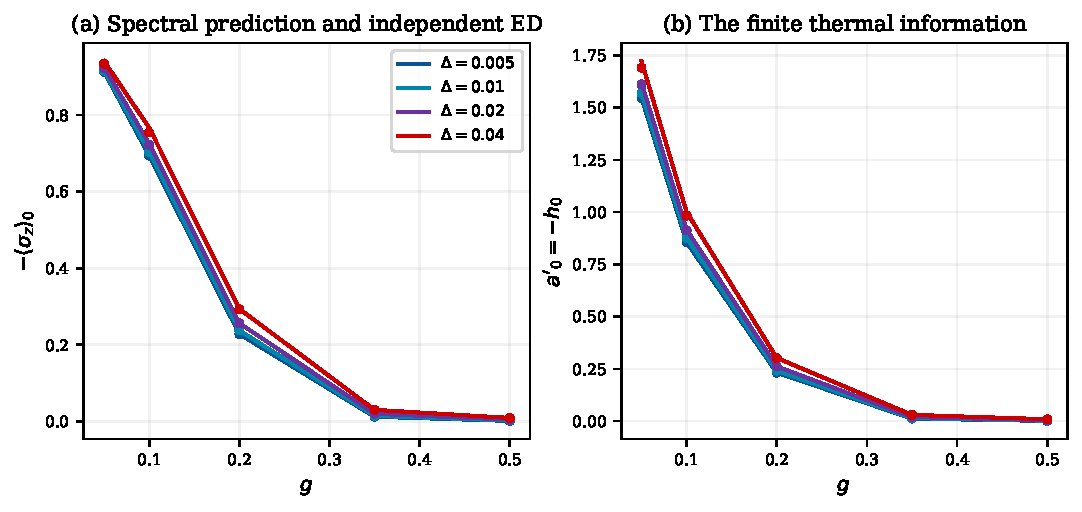
\includegraphics[width=\linewidth]{../figures/generated/dd-hmf-physical-ground-state-20261016.pdf}
\caption{The bath spectrum predicts the cold spin before numerical comparison.~\cite{McCaul2026e37796} (a) Lines show $-\langle\sigma_z\rangle_0=S_g+\Delta A_g$ and points show independent diagonalisation of the original Hamiltonian, with $\sigma_z=-\tau_x$. (b) The normalised conditional-bath trial predicts the dimensionless thermal coordinate $a'_0=-h_0$, compared with the coordinate obtained from those numerical ground states. Here $h_0=-\operatorname{arctanh}r_0$, where $r_0$ is the reduced spin's Bloch-vector length. The two bath energies are $\nu_k=(0.2,1.8)$ and $v_k^2=4\nu_k e^{-\nu_k/2}$ in the chosen energy unit. The legend gives the tunnelling energy $\Delta$ and the horizontal axis the coupling $g$. Bath coupling is retained exactly, while tunnelling is controlled relative to the fixed bath gap. The comparison includes two oscillator cutoffs and a separate joint-vector check.}
\label{fig:dd-hmf-physical-ground-state-20261016}
\end{figure}

\subsection{Carry the answer back}
In the original energy axes, $\sigma_z=-\tau_x$. With $r_0=S_g+\Delta A_g+O(\Delta^2)$, the reduced ground state is $\rho_0=(I-r_0\sigma_z)/2$. Its eigenvalues $(1\pm r_0)/2$ specify the local probabilities and entropy. More generally, the three spin averages form the Bloch vector $\mathbf m$ in $\rho=(I+\mathbf m\cdot\boldsymbol\sigma)/2$, where $\boldsymbol\sigma$ denotes the three Pauli spin matrices. Cooling the composite therefore need not make the subsystem pure: its entanglement with the displaced bath survives. The dimensionless coordinate $h_0=-\operatorname{arctanh}r_0$ records the corresponding population imbalance. The dual-reference construction carries this predicted state to a finite reference coordinate $a'_0=-h_0$. Here $a'=\beta'\omega'_r/2$ is half the chosen reference splitting $\omega'_r$ in units of its temperature. The endpoint is shown in Fig.~\ref{fig:dd-hmf-physical-ground-state-20261016}(b).

A reference change must preserve more than the appearance of a normalised matrix. Let $\mathcal R=R_S/Z_B$ be the unnormalised mean-force operator from Eq.~\eqref{eq:mean-force-normalised}. Factor it as $\mathcal R=G_b\Xi_bG_b$, where $G_b$ is a strictly positive reference thermal factor and $\Xi_b$ the remaining influence. For another strictly positive factor $G_r$, define
\begin{equation}
 A=G_r^{-1}G_b,\qquad
 \Xi_r=A\Xi_bA^\dagger,\qquad
 G_r\Xi_rG_r=\mathcal R,\qquad
 \langle O\rangle=
 \frac{\operatorname{Tr}(\Xi_rG_rOG_r)}
      {\operatorname{Tr}(\Xi_rG_r^2)}.
 \label{eq:hmf-reference-transport}
\end{equation}
At finite temperature this identity retains the full operator. In taking its cold limit, the scalar ground-energy factor $e^{-\beta E_0}/Z_B$ accompanies the limiting reduced state. The denominator retains the partition weight, the numerator the measured observable $O$. Their order matters when the factors do not commute. A convenient reference for a predicted state with Bloch vector $\mathbf m_0$ points along $\mathbf n_r=-\mathbf m_0/|\mathbf m_0|$. The state is diagonal along this adapted axis, while the axis itself retains its physical orientation. In the mixed case $0<|\mathbf m_0|<1$, its finite coordinate is again $a'_{r,0}=\operatorname{arctanh}|\mathbf m_0|$. This transports the answer already calculated from the bath, including its scalar weight and observable interpretation.~\cite{McCaul2026e37796}

This suggests a concrete route to better machine-learning calculations. When a difficult interaction is already understood, represent it explicitly before asking an optimiser to learn or correct everything else. The remaining operator should expose a bounded correction, a useful spectrum or a measurable residual. The loss-operator diagnostics in the next section retain directions that a scalar objective hides. Gap-aware trial-space enlargement spends effort on omitted directions according to their effect on the answer. Task-directed memory retains the relations needed to reconstruct a query. The spin--bath calculation supplies a physical example of the same strategy with an analytic error control. Transferring it to a learning problem means identifying that problem's solvable structure, pricing the transformation and checking the reconstructed predictions against a matched-cost baseline. It is a method for designing and testing improved calculations, rather than a speed-up inferred merely from using quantum notation.

\subsection{When refinement changes the questions}
The reference transformation above preserves the same physical state. Changing resolution poses a different problem: the resolved distinctions themselves may change. This is the second thread developed in The Law of Laws, where quantum-like structure can appear when successive descriptions lose information in a way that cannot be absorbed into a change of scalar costs. The preceding closure residual tells us that a retained state is missing part of its evolution. Now ask whether refining that description merely changes the values attached to its resolved modes, or also changes which directions count as distinct modes. The latter requires an operator account of the change.

Foundations develops this question in \emph{Transporting a spectral description}, within Chapter 3's discussion of where discarded information went.~\cite{Reference0e02fc} To compare neighbouring descriptions, first specify a common inner-product space of fixed dimension and how its coordinates are transported. Write $\mathsf K_s$ for a differentiable Hermitian effective operator at description parameter $s$, and $\mathsf J_s$ for the anti-Hermitian generator of the chosen frame transport. Hermitian means equal to its conjugate transpose, while anti-Hermitian means its negative. The transport preserves inner products. We use different letters here from the probability generator $G$ and coarse map $C$: this is a smooth, fixed-rank comparison of the resolved operators.

An infinitesimal comparison map is $T_{s\to s+h}=I+h\mathsf J_s+o(h)$. The difference between transporting the old law and applying the new law is
\begin{equation}
 T_{s\to s+h}\mathsf K_s-\mathsf K_{s+h}T_{s\to s+h}
 =h\omega_s+o(h),\qquad
 \omega_s=[\mathsf J_s,\mathsf K_s]-\mathsf K'_s .
 \label{eq:refinement-residue-density}
\end{equation}
Here $[A,B]=AB-BA$, the prime denotes differentiation with respect to $s$, and $o(h)$ denotes terms smaller than first order as $h\to0$. The finite-step mismatch tends to zero as the step shrinks, but its density $\omega_s$ can remain nonzero. That is the quantity to follow through increasingly fine descriptions.

The distinction between diagonal and off-diagonal residue is the mechanism. Let $\lambda_i$ be a simple eigenvalue of $\mathsf K_s$ and $\Pi_i$ its spectral projector. Differentiating the eigenvalue equation gives
\begin{equation}
 \Pi_j\bigl(\Pi_i'-[\mathsf J_s,\Pi_i]\bigr)\Pi_i
 =-\frac{\Pi_j\omega_s\Pi_i}{\lambda_i-\lambda_j},
 \qquad j\ne i .
 \label{eq:refinement-projector-rotation}
\end{equation}
Diagonal residue shifts eigenvalues. Off-diagonal residue rotates the spectral directions after the chosen coordinate transport has been removed. A small gap allows a given mismatch to rotate those directions strongly. Merely adjusting a list of scalar penalties cannot describe that rotation.

For a fixed-coordinate example, choose $\mathsf J_s=0$ and a resolved direction $u_s=(\cos\nu s,\sin\nu s)^T$, with projector $\Pi_s=u_su_s^T$ and fixed nonzero rotation rate $\nu$. At $s=0$,
\[
 \lim_{h\to0}\frac{[\Pi_0,\Pi_h]}h
 =\nu\begin{pmatrix}0&1\\-1&0\end{pmatrix}.
\]
The projectors themselves become arbitrarily close as $h$ shrinks, yet in this fixed frame the rate at which their order matters stays finite. A co-rotating frame could remove this example's rotation. A residual claim therefore depends on which coordinate transport the comparison admits. Law of Laws~\cite{McCaulad9572} proposes a self-similar regime in which off-diagonal residue remains significant relative to the spectral gap. The effective description then keeps a noncommuting algebra of resolved distinctions instead of settling into one fixed spectral basis. This is the precise quantum-like feature that the refinement argument brings into the programme.

Foundations places that feature beside two further constructions. Chapter 2 tests whether overlapping measurement contexts admit one global assignment, while Chapter 3 exhibits classical averaging and reversible Markov examples with noncommuting operations or rotating eigenspaces. The distinction is productive: the spectral calculation identifies the persistent operator structure, and the context experiment asks which probability accounts it can support. This is an author-proposed connection. Connecting these constructions into a physical quantum reconstruction requires the specified event algebra, composition and measurement rule, as well as a calibrated action scale. These conditions specify the next reconstruction problem.

\subsection{Can the retained questions share one probability account?}
The four-state example asks whether a summary can carry a prediction forward in time. A different test is whether several summaries can be combined into one consistent account. Here the information at risk is which observations belong together. A \emph{context} is a set of measurements that can be made jointly. If an observable belongs to two contexts, its identity must remain the same in both. Foundations Chapter 2 asks whether the joint probability tables for overlapping contexts can all be obtained as marginals of one context-independent distribution.~\cite{McCaul85986c}

The two-qubit Peres--Mermin construction makes the obstruction elementary. In a two-state basis the Pauli matrices are
\[
 X=\begin{pmatrix}0&1\\1&0\end{pmatrix},\quad
 Y=\begin{pmatrix}0&-i\\i&0\end{pmatrix},\quad
 Z=\begin{pmatrix}1&0\\0&-1\end{pmatrix}.
\]
Here $i^2=-1$ and $I$ is the identity. For two qubits, $X\otimes I$ acts on the first and $I\otimes X$ on the second. Arrange the observables as
\[
 \begin{array}{ccc}
 X\otimes I&I\otimes X&X\otimes X\\
 I\otimes Z&Z\otimes I&Z\otimes Z\\
 X\otimes Z&Z\otimes X&Y\otimes Y
 \end{array}.
\]
Within each row or column the three matrices commute, so their joint outcome constraints can be tested.  Each has outcomes $+1$ or $-1$, and every row and column is a jointly measurable context. The operator products require
\[
 \begin{array}{c|ccc}
 \text{context}&1&2&3\\ \hline
 \text{row product}&+1&+1&+1\\
 \text{column product}&+1&+1&-1
 \end{array}.
\]
Suppose one value could be assigned to every cell independently of how it was measured. Multiplying all six context products would use each cell twice, giving $+1$. The required signs instead multiply to $-1$. At least one context constraint must fail. If $W$ counts agreement with each required sign as $+1$ and disagreement as $-1$, every such assignment and every probability mixture obeys $W\le4$, while the quantum product identities give $W=6$. The displayed operators specify the sign constraints without requiring a companion derivation. The crucial retained information is the overlap of measurement identities, not merely six unrelated summaries.

This is different from the dynamical closure residual: one tests a common probability account, the other tests autonomous evolution of a retained state. A change of coordinates or frame can change the matrices used to describe the same observables without changing their predictions. That freedom of representation must be distinguished from changing a measurement context, which changes the jointly accessible questions. The spectral-transport construction above makes one such frame comparison explicit. Together these connect retained distinctions, overlapping measurement contexts and changes of spectral frame.

\subsection{A loss with specified dynamics}
The changing spectral directions show why an operator can carry information that scalar costs alone miss. To use that idea in a calculation, we need a specified motion as well as a cost landscape. A stochastic dynamics supplies a concrete construction. Consider a coordinate moving down a smooth confining potential $V(x)$ while receiving random kicks:
\begin{equation}
 dX_t=-V'(X_t)\,dt+\sqrt{2T}\,dW_t,
 \qquad
 \partial_t p=\partial_x(V'p)+T\partial_x^2p.
 \label{eq:loss-diffusion}
\end{equation}
$W_t$ is standard Brownian motion and $T>0$ sets the noise intensity. Mobility has been set to one. With appropriate boundary conditions, the stationary density is $\pi(x)=Z^{-1}e^{-V(x)/T}$. Writing $p(x,t)=\sqrt{\pi(x)}\,\psi(x,t)$ transforms the evolution into
\begin{equation}
 T\partial_t\psi=-H_V\psi,\qquad
 H_V=-T^2\partial_x^2+\frac{(V')^2}{4}-\frac{T V''}{2}.
 \label{eq:loss-operator}
\end{equation}
This is a change of representation with a clear gain. The original density evolution becomes a self-adjoint spectral problem under the corresponding domain and boundary conditions. The weighted density norm $\int |p|^2/\pi\,dx$ becomes the ordinary squared norm of $\psi$. Relaxation modes can now be studied with operator methods.~\cite{Reference0e02fc}

The factor $T$ on the left is essential. For $V(x)=\kappa x^2/2$, the operator eigenvalues are $E_n=n\kappa T$, while the decay rates are $E_n/T=n\kappa$. Confusing the eigenvalues with rates would change the physical time scale. The stationary mode is $\psi_0=\sqrt{\pi}$ and has zero eigenvalue. This construction belongs to the established relationship between diffusion, factorised operators and supersymmetric quantum mechanics, developed mathematically in Witten's work.\footnote{E. Witten, \emph{Supersymmetry and Morse Theory}, Journal of Differential Geometry 17 (1982),661--692, \href{https://doi.org/10.4310/jdg/1214437492}{doi:10.4310/jdg/1214437492}.} Its role here is operational: a loss landscape and specified noise law supply an operator whose low modes describe relaxation.~\cite{Witten1982605ee8}

\subsection{Keep a useful correction visible}
The choice of objective can be just as consequential as the choice of dynamics. Suppose $n$ independently controlled two-level components should all end in their preferred state, and component $j$ succeeds with probability $p_j=\cos^2(\theta_j/2)$. Two losses have exactly the same perfect solution:
\begin{equation}
 C_G=1-\prod_{j=1}^n p_j,\qquad
 C_L=1-\frac{1}{n}\sum_{j=1}^n p_j.
 \label{eq:global-local-cost}
\end{equation}
The global loss rewards the complete conjunction. The local loss rewards each corrected component. For independently uniform angles, their derivative variances are
\begin{equation}
 {\rm Var}(\partial_j C_G)=\frac18\left(\frac38\right)^{n-1},
 \qquad
 {\rm Var}(\partial_j C_L)=\frac{1}{8n^2}.
 \label{eq:global-local-variance}
\end{equation}
A global demand can thus bury a useful local signal exponentially fast even when the answer itself is unchanged. Figure~\ref{fig:dd-global-local-feedback} makes the difference visible. Cerezo and colleagues use this example to distinguish cost-dependent concentration from the broader random-circuit barren-plateau mechanism established by McClean and colleagues.\footnote{M. Cerezo et al., \emph{Cost function dependent barren plateaus in shallow parametrized quantum circuits}, Nature Communications 12 (2021), \href{https://doi.org/10.1038/s41467-021-21728-w}{doi:10.1038/s41467-021-21728-w}. J. R. McClean et al., \emph{Barren plateaus in quantum neural network training landscapes}, Nature Communications 9 (2018), \href{https://doi.org/10.1038/s41467-018-07090-4}{doi:10.1038/s41467-018-07090-4}.} Locality is a design resource, not a guarantee that arbitrarily deep or poorly conditioned models train easily.~\cite{Cerezo2021232f10,McClean20183bd480}
\begin{figure}[htbp]
\centering
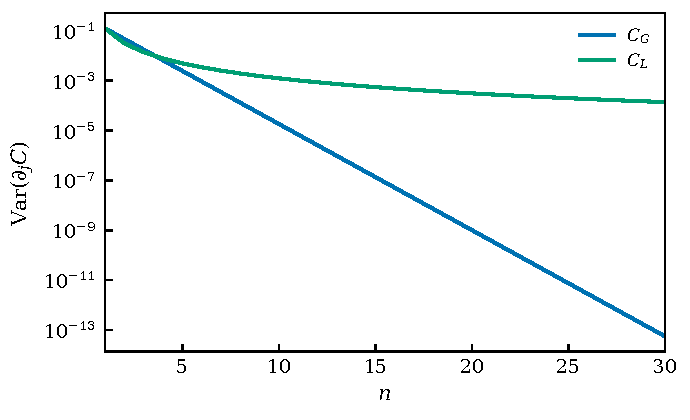
\includegraphics[width=\linewidth]{figures/portable-run-b69220b3a27348ad.result/dd-global-local-feedback.pdf}
\caption{The same optimum with different feedback. For the product-state example of Cerezo et al.~\cite{Cerezo2021232f10}, the global and local losses in Eq.~\eqref{eq:global-local-cost} have the same zero-cost target. With independent uniform angles, $\operatorname{Var}(\partial_j C_G)=\tfrac18(\tfrac38)^{n-1}$, while $\operatorname{Var}(\partial_j C_L)=1/(8n^2)$. Here $n$ is the number of qubits. Exact model variances isolate cost-dependent concentration.}
\label{fig:dd-global-local-feedback}
\end{figure}

\subsection{Combining local responses without instability}
Usable feedback needs more than a visible signal. Combining many responsive components can also make a correction too strong. Adaptive Normal Form and Phases of Hierarchy study this stability problem. In the latter's sampled model, a plant state $x_k$ relaxes towards $s\theta_k$ between updates,
\[
 x_{k+1}=r x_k+(1-r)s\theta_k,\qquad
 e_k=x_{k+1}-b\theta_k,\qquad
 \theta_{k+1}=\theta_k+\alpha R_N(e_k).
\]
Here $r=e^{-h/\tau_r}$ is the fraction of the previous state retained over sampling interval $h$, $\tau_r$ the relaxation time, $s$ the plant gain, $b$ the reference gain, and $\alpha$ the update size. The response of a noisy majority of $N$ components is approximated by
$R_N(e)\simeq{\rm erf}(\beta e\sqrt{N/2})$, so its small-signal slope is $G_N\simeq\beta\sqrt{2N/\pi}$. Increasing $N$ increases the loop gain $K=\alpha G_N$.

For $0<r<1$ and $b>s>0$, the linearised discrete dynamics is stable only when
\begin{equation}
 0<K<
 \frac{2(1+r)}{(1+r)b-(1-r)s}.
 \label{eq:feedback-bound}
\end{equation}
In the declared example, $\alpha=0.35$, $\beta=0.6$, $b=1.2$, $s=0.4$ and $r=e^{-1}$ put the Gaussian-response crossing near $N=138.25$. Adding responsive components can therefore destabilise a loop whose individual parts have not changed. The boundary quantifies the permitted response gain in this sampled loop.~\cite{McCaul630942}

The hierarchy in Phases of Hierarchy makes that change explicit. Let layer $\ell$ combine $n_\ell$ inputs, so $L$ aggregation layers represent $N=\prod_{\ell=1}^L n_\ell$ bottom-level components. In the paper's iterated Gaussian approximation, the expected response obeys $m_\ell(e)=\operatorname{erf}(\sqrt{n_\ell/2}\,m_{\ell-1}(e))$, with individual slope $m_0'(0)=\beta$. Differentiating each stage at zero and multiplying its slopes gives
\begin{equation}
 K_N^{(L)}=\alpha\beta\sqrt{\frac{2N}{\pi}}\,c^{L-1},
 \qquad c=\sqrt{\frac{2}{\pi}},
 \qquad
 N_c^{(L)}=N_c^{(1)}\left(\frac{\pi}{2}\right)^{L-1}.
 \label{eq:hierarchy-stability}
\end{equation}
Here $L=1$ is the flat aggregate. The factor $c$ is attenuation relative to a flat group of the same total size, not the absolute gain of each local block. One more aggregation layer therefore raises the population threshold by $\pi/2$ within this model. Figure~\ref{fig:dd-hierarchy-stability} shows the resulting phase diagram: a population of $200$ lies beyond the flat threshold but below the two-layer threshold at $\alpha=0.35$ and $h/\tau_r=1$. Slower updates provide another way to remain stable because the plant has longer to relax before the next correction.~\cite{McCaul630942}

Attenuating a response also has a cost. In the paper's separate depth-$L$ linear control cascade with attenuation $0<c<1$, the minimum squared-input effort needed to produce a unit apex response scales as $c^{-2(L-1)}$, once the control horizon is long enough to reach the apex. The cascade provides a separate measure of the intervention cost of attenuation. Adaptive Normal Form supplies a related gradient-feedback construction, but its effective gain contains two response derivatives and scales differently.~\cite{McCaul74663e} The common design question is where an aggregate response should be represented and acted upon, with its stability, signal and control costs accounted for.
\begin{figure}[htbp]
\centering
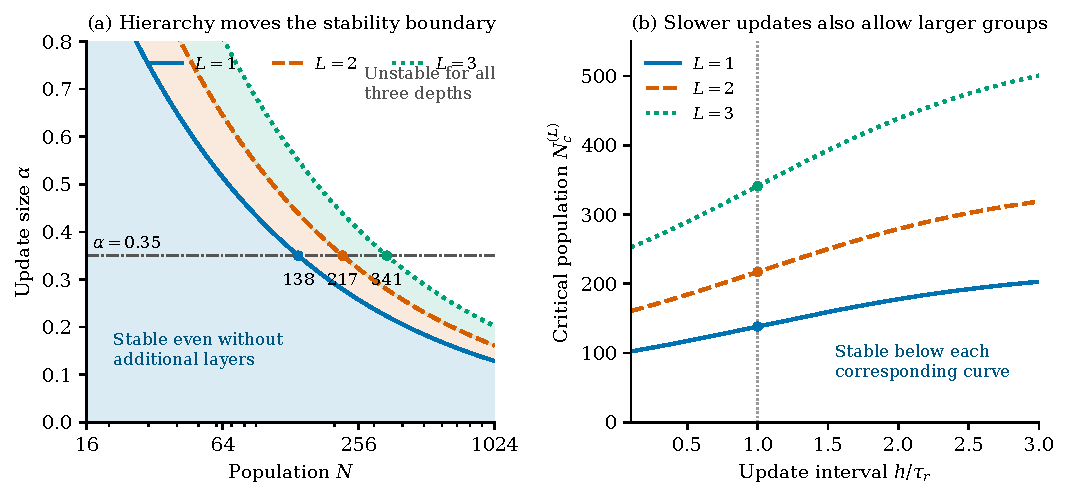
\includegraphics[width=\linewidth]{figures/hierarchy-run-d9f38e92caf64d82.result/dd-hierarchy-stability.pdf}
\caption{Hierarchy moves the stability boundary of the sampled feedback model. (a) At $h/\tau_r=1$, each curve separates stable dynamics below it from instability above it. The orange and green bands show additional parameter ranges stabilised by a second and third aggregation layer. The $\alpha=0.35$ slice crosses at $N_c^{(1)}=138.25$, $N_c^{(2)}=217.17$ and $N_c^{(3)}=341.13$. (b) At fixed $\alpha=0.35$, increasing the update interval also raises the critical population. In both panels $\beta=0.6$, $b=1.2$ and $s=0.4$. Curves use the iterated Gaussian expected-majority model of Phases of Hierarchy~\cite{McCaul630942}, not exact small-block voting or ANF's different feedback rule. The numerical checks of the linear boundary are retained with the figure's result record.}
\label{fig:dd-hierarchy-stability}
\end{figure}

These examples give representation a more demanding meaning than a relabelling of variables. A retained coordinate determines which history must be carried. A loss determines which corrections remain visible. A feedback architecture determines how many local responses can be combined without losing stability. The practical question is then whether these distinctions can guide a calculation that would otherwise be unnecessarily difficult.


\section{Quantum prototypes: changing the calculation}
\label{section:quantum-prototypes-changing-the-calculation}

The preceding examples show how representation changes the information available to a calculation. The next test is operational: can we use that information to choose better updates, trial states or measurements? We examine three operational methods: inspect feedback before its scalar projection, repair the retained trial space, and choose a spectral window whose measurements remain informative.

A pure quantum state is a vector of complex amplitudes. Their squared magnitudes give outcome probabilities in a chosen measurement basis. An observable is a Hermitian operator, and its expectation value is the average score obtained by repeatedly preparing and measuring the state. A Hamiltonian $H$ is the observable for energy. Finding its lowest-energy state is useful in molecular and materials calculations, but a general $n$-qubit state has $2^n$ amplitudes. The choice of accessible states and measurements is therefore central to the calculation.

The circuit $U$ preserves the state vector's norm. Its adjustable gates determine which states the calculation can prepare.

A variational algorithm prepares a family of states $|\psi(\theta)\rangle=U(\theta)|\psi_0\rangle$ using a parameterised circuit $U$, measures an energy or other cost, and adjusts $\theta$. It combines a quantum experiment with a classical optimiser. There are at least three different ways for this procedure to struggle. The measured scalar can conceal a useful operator change. The chosen trial family can omit the needed state. The measurement used to resolve a spectral feature can become ill-conditioned. The Eigen prototypes make those failures distinct and suggest a different repair for each.

Three operators now have distinct jobs. The differential operator $H_V$ in Eq.~\eqref{eq:loss-operator} describes relaxation of a classical density. The circuit loss operator $\mathcal L(\theta)$ describes the changing quantum observable. The Hamiltonian $H$ in the residual calculation describes the physical system whose low-energy state we seek. Spectral analysis is useful in each of these spaces.

\subsection{Operator diagnostics before scalar feedback}
The loss-operator construction starts before the scalar reading.~\cite{McCaul0c5ec5}

\begin{equation}
 {\cal L}(\theta)=U(\theta)^\dagger O U(\theta),\qquad C(\theta)=\langle\psi_0|{\cal L}(\theta)|\psi_0\rangle.
 \label{eq:operator-scalar}
\end{equation}
$O$ is the measured observable, the dagger denotes the conjugate transpose, and ${\cal L}$ retains the circuit's action on the observable. The scalar $C$ samples it with one input state. This is the familiar Heisenberg representation used for a particular purpose: distinguish information in the changing operator from the training signal exposed by one measurement functional.

At a differentiated gate, the gradient can be written as $\langle\psi|A|\psi\rangle$ for a Hermitian traceless operator $A=(i/2)[G,\Omega]$, where $G$ generates that gate, $\Omega$ is the appropriately propagated observable and $[G,\Omega]=G\Omega-\Omega G$. For a fixed $A$, if the state is drawn independently of $A$ from a state 2-design, meaning that its second moments match those of a uniformly random pure state, then
\begin{equation}
 {\rm Var}\big(\langle\psi|A|\psi\rangle\big)=\frac{{\rm Tr}(A^2)}{d(d+1)},\qquad d=2^n.
 \label{eq:operator-variance}
\end{equation}
The squared Hilbert--Schmidt norm is $\|A\|_{\rm HS}^2=\operatorname{Tr}(A^\dagger A)$. The operator can retain substantial squared norm while its scalar reading concentrates. For a Pauli observable with squared Hilbert--Schmidt norm $d$, a normalised gradient-operator fraction near one half gives variance near $1/[2(d+1)]$. The normalisation explains the scaling rather than hiding it.

The archived fixed-operator checks and two-to-eight-qubit circuit ensembles test this distinction directly. Figure~\ref{fig:dd-operator-projection} shows the scalar-gradient variance falling while the normalised operator-gradient fraction remains near one half. The local and global observable ensembles behave similarly here. The calculation explains how a substantial operator change can become difficult to see through a single scalar measurement.
\begin{figure}[htbp]
\centering
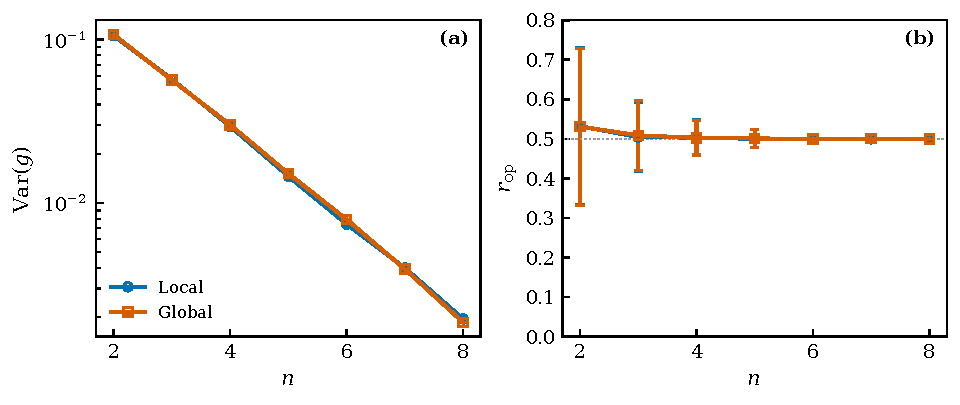
\includegraphics[width=\linewidth]{figures/portable-run-b69220b3a27348ad.result/dd-operator-projection.pdf}
\caption{Operator content and scalar feedback. Archived classical circuit-ensemble calculations, seed 20240603 and 2,000 samples per point. (a) Scalar-gradient variance $\operatorname{Var}(g)$ decreases with qubit number $n$. (b) The normalised operator-gradient fraction $r_{\rm op}=\|A\|_{\rm HS}^2/\|O\|_{\rm HS}^2$ remains near one half. Bars are archived sample standard deviations, not confidence intervals. The local and global observable ensembles nearly coincide in this experiment. The comparison isolates the scalar-projection mechanism. Measuring the operator content remains a separate resource cost.}
\label{fig:dd-operator-projection}
\end{figure}

The next design question is where that operator content sits. A Pauli string is a tensor product of the one-qubit identity and Pauli matrices $I,X,Y,Z$. For example, $X$ exchanges the two basis states and $Z$ reverses the sign of the second amplitude. Its weight counts the nonidentity factors: $Z_1X_2$, for example, has weight two. Expanding the operator in these strings groups contributions by the number of qubits on which they act. Keeping low-weight content can make measurements or local constructions manageable. The source experiments track how those bands change with circuit depth. Their useful implication is diagnostic: inspect what a scalar projection has obscured before attributing every failure to the optimiser. The tested block-and-merge training hierarchy did not outperform a deep global optimiser on the reported models up to ten qubits. The stronger practical construction comes from using a residual to change the trial representation itself.

\subsection{Residual-guided active-space repair}
The active-space repair is developed in Closure-Guided Active-Space Repair for Variational Quantum Algorithms.~\cite{McCaul8cce8c} Let $P$ be the orthogonal projector onto a retained linear state space and $Q=I-P$ onto the omitted space. Suppose the lowest eigenproblem inside $P$ has been solved, producing a normalised Ritz state $\phi$ and energy $E$:
\begin{equation}
 PHP\phi=E\phi,\qquad r=Q(H-E)\phi=QH\phi,\qquad \|r\|^2=\langle\phi|(H-E)^2|\phi\rangle.
 \label{eq:ritz-residual}
\end{equation}
The residual $r$ is the part of the full eigenvalue equation that remains unsatisfied. The internal optimiser has finished its task. Repeating that same optimisation cannot lower the minimum available inside $P$. Enlarging or rotating the retained space can.

For a normalised omitted direction $w$, write $a=\langle w|r\rangle$ and $\beta=\langle w|H|w\rangle$. Solving the two-dimensional problem on $\mathrm{span}\{\phi,w\}$ gives
\begin{equation}
 e_-=\frac{E+\beta-\sqrt{(\beta-E)^2+4|a|^2}}{2},\qquad E_{\rm enlarged}\leq e_-.
 \label{eq:ritz-descent}
\end{equation}
A nonzero overlap $a$ guarantees a strict decrease relative to $E$. The inequality matters: the whole enlarged space may do better than this two-dimensional restriction. When $\beta-E>0$ is large compared with $|a|$, the estimated gain is $|a|^2/(\beta-E)$. A larger discrepancy is not necessarily a more valuable correction if reaching it costs much more energy.

The exact block elimination behind this reasoning is the Feshbach effective operator
\begin{equation}
 H_F(E)=PHP+PHQ(E-QHQ)^{-1}QHP.
 \label{eq:feshbach}
\end{equation}
The inverse acts on the omitted space $\operatorname{Ran}(Q)$ and the expression applies where that inverse exists. In a full eigenpair, the omitted component is obtained by applying $(E-QHQ)^{-1}QHP$ to the retained component. Replacing that unknown full solution by a Ritz pair gives a practical correction approximation. The denominator supplies physical information that the raw residual alone does not contain.

The four-qubit rank-growth prototype uses
\[
 H_{\rm grow}(\lambda)=-X_0-0.7X_1+0.2Z_0Z_1
 +4(n_2+1.2n_3)+\lambda(Z_1X_2+0.7X_0X_3),
 \quad n_j=(I-Z_j)/2.
\]
Here $n_j$ penalises excitation of qubit $j$ and $\lambda$ sets the coupling to the initially omitted qubits. The initial rank-four space allows two qubits to vary and fixes the other two. At $\lambda=1$, adding two residual directions reduces the energy error by almost three orders of magnitude. A restricted pool of one- and two-qubit Pauli directions also gives a substantial improvement, and both routes reach numerical roundoff by rank ten. These exact dense-state calculations expose the effect of enlarging the representation before finite-shot measurement costs enter.

For the two-channel comparison in Figure~\ref{fig:dd-gap-selection}, the model is
\begin{align}
H(\lambda)={}&-X_0-0.7X_1+0.2Z_0Z_1+0.4n_2+30n_3\nonumber\\
 &+\lambda(0.8Z_1X_2+0.9X_0X_3),\qquad n_j=(I-Z_j)/2 .
\end{align}
The operator $n_j$ penalises excitation of qubit $j$. Initially qubits 0 and 1 vary, while qubits 2 and 3 remain in $|00\rangle$. The candidate pool contains the two displayed boundary operators. One excites a cheap omitted degree of freedom, the other an expensive one. This is a separate multiscale test from the preceding rank-growth example.

The multiscale example separates the size of a coupling from the benefit of following it. The channel with the larger raw overlap is much more expensive to excite. The smaller-overlap, low-gap direction therefore produces the larger energy decrease. Figure~\ref{fig:dd-gap-selection} compares the resulting errors across coupling strengths: denominator-aware selection spends the same extra direction where it changes the answer most.
\begin{figure}[htbp]
\centering
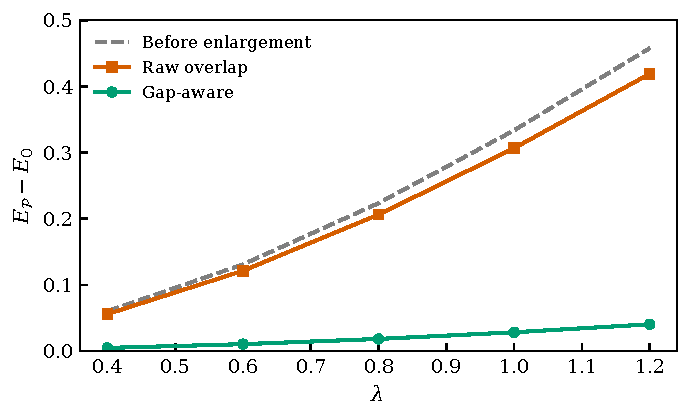
\includegraphics[width=\linewidth]{figures/portable-run-b69220b3a27348ad.result/dd-gap-selection.pdf}
\caption{Choose an omitted direction by its value, not only its amplitude. Each method adds one direction from the same pool in the archived residual prototype. Coupling $\lambda$ and retained-space energy error $E_P-E_0$ use the model's dimensionless units. Raw residual amplitude favours a high-gap channel. The implemented amplitude-over-gap rule selects a more useful low-gap channel and leaves a smaller error. The curves are exact dense-state calculations for the displayed Hamiltonian and two-candidate pool.}
\label{fig:dd-gap-selection}
\end{figure}

For normalised candidates, the implemented amplitude-over-gap score is $|a|/|\beta-E|$. The second-order energy-gain estimate is $|a|^2/(\beta-E)$ when $\beta-E>0$ is large compared with $|a|$. These are different rankings in general, although both select the useful channel here. Their distinction belongs in the reproducible algorithm specification. The relevant prior comparison is ADAPT-VQE, which already grows an ansatz by testing a pool of candidate operators. Its original ranking uses energy gradients rather than an energy denominator, and it trades a more compact circuit for extra pool measurements.\footnote{H. R. Grimsley et al., \emph{An adaptive variational algorithm for exact molecular simulations on a quantum computer}, Nature Communications 10 (2019), \href{https://doi.org/10.1038/s41467-019-10988-2}{doi:10.1038/s41467-019-10988-2}.} Eigen's residual examples motivate a testable improvement in selection, not a claim to have invented adaptive ansatz growth.~\cite{Grimsley20198f59be}

There is also a revealing success at the end of the rank-growth calculation. The target state's residual becomes negligible while the whole-space leakage $\|QHP\|$ remains finite. The desired eigenstate has been captured, but the retained space is not invariant for every state it contains. A zero residual by itself certifies an eigenpair, not the ground state: for $H=\operatorname{diag}(0,1)$ and $P$ retaining only the second coordinate, the lowest-in-$P$ pair has $E=1$ and $r=0$, while the true ground energy is zero. Ground-state certification therefore needs an additional bound or spectral condition. This is precisely the task-relative distinction introduced by the four-state process. Fidelity to the required answer can be cheaper than closure of the whole description.

\subsection{Spectral windows with reusable measurements}
Spectral estimation asks a related question about resolution rather than trial-space size. For a probe energy $\lambda$ and $\tau>0$, define
\begin{align}
 Z_\tau(\lambda)&=\langle\psi_0|e^{-\tau(H-\lambda)^2}|\psi_0\rangle,\nonumber\\
 N_\tau(\lambda)&=\langle\psi_0|H e^{-\tau(H-\lambda)^2}|\psi_0\rangle,\qquad F_\tau=\frac{N_\tau}{Z_\tau}.
 \label{eq:spectral-filter}
\end{align}
The Gaussian selects energies within a width of order $\tau^{-1/2}$ around $\lambda$. $F_\tau$ is their weighted mean. Moving the window traces supported spectral levels. An eigenvalue with zero input-state weight remains invisible to this expectation.

For a self-adjoint $H$, the exact Fourier identity
\begin{equation}
 e^{-\tau(H-\lambda)^2}=\frac{1}{\sqrt{4\pi\tau}}\int_{-\infty}^{\infty}e^{-s^2/(4\tau)}e^{-is(H-\lambda)}\,ds
 \label{eq:gaussian-fourier}
\end{equation}
expresses the filter through real-time unitary evolution. Quantum hardware naturally implements those rotations. The probe energy enters as a classical phase, so the same measured overlaps can be reweighted for several windows. Figure~\ref{fig:dd-spectral-window} explains this reuse. A narrower energy question requires longer time information and more precise estimation, not merely a different label on the plot.
\begin{figure}[htbp]
\centering
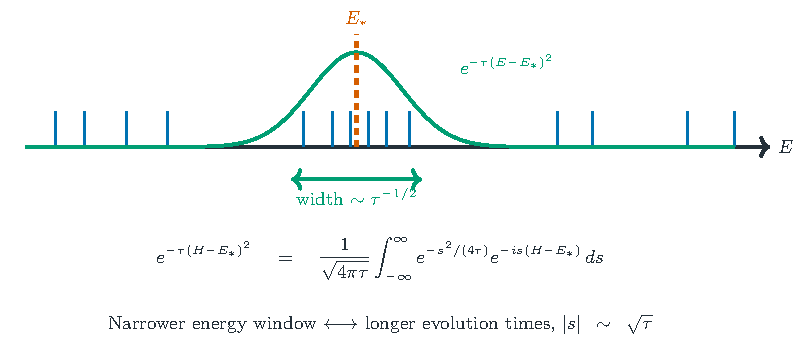
\includegraphics[width=\linewidth]{figures/portable-run-b69220b3a27348ad.result/dd-spectral-window.pdf}
\caption{A spectral window and its time-domain cost. For self-adjoint $H$, real probe energy $E_\star$ and $\tau>0$, the Gaussian width scales as $\tau^{-1/2}$. The Fourier representation uses real-time evolution on a scale proportional to $\sqrt{\tau}$, with $\hbar=1$. Here $E_\star$ is the probe denoted $\lambda$ in Eq.~\eqref{eq:spectral-filter}. Narrower resolution requires longer-time information. ITQDE supplies the overlap construction, while Free Snacks examines local support and conditioning. This is a mathematical schematic, not a measured spectrum.}
\label{fig:dd-spectral-window}
\end{figure}

Quantum Dynamical Emulation of Imaginary Time Evolution, or ITQDE, provides a concrete measurement construction. It reconstructs filtered expectations from forward/backward overlaps using ancilla-assisted tests. The paper includes a two-system-qubit IBM Brisbane experiment with 104 random Clifford initial states and 4,000 samples per overlap, alongside separate numerical and simulator examples. This is evidence that the overlap route can be implemented on hardware at that scale. Its economy is reuse and reduced coherent-circuit requirements, paid for with sampling rather than free preparation of a filtered state.~\cite{Leamer20249db941}

Free Snacks in Quantum Complexity~\cite{McCaul2025f7b569} focuses on when the ratio becomes unreliable. With estimated errors $\delta N,\delta Z$ and $|\delta Z|<Z$, elementary rearrangement gives
\[
 |\widehat F-F|\leq\frac{|\delta N|+|F|\,|\delta Z|}{Z-|\delta Z|}.
\]
A narrow window placed between widely separated supported levels has a small denominator. Even accurate overlap estimates can then give an unstable ratio. Within the paper's additive-noise model, resolving a very small gap while crossing a large one can demand a rapidly growing sample budget. The relevant bandwidth is a ratio of scales in the chosen spectral window, not simply the total number of qubits.

Local coarsening offers a controlled response. Convolving the numerator and denominator separately in probe energy with a normalised Gaussian of variance $\sigma^2$ gives a common prefactor $(1+2\tau\sigma^2)^{-1/2}$ and replaces $\tau$ by $\tau/(1+2\tau\sigma^2)$. The prefactor cancels in their ratio. This square-completion calculation uses separate numerator and denominator smoothing, which is generally different from smoothing their ratio. Existing overlap data can therefore answer a coarser question without rerunning a separate circuit for every probe energy. The price is merging distinctions. Whether that is acceptable depends on the observable or decision being sought.

Together, these prototypes supply a practical programme. Preserve the operator information that a scalar reading hides. Add omitted directions according to their expected value, not merely their magnitude. Choose spectral resolution where the estimator can support it. Candidate preparation, measurements, optimisation and conditioning then belong in one cost comparison. The same design problem appears when the large object is a collection of records rather than a quantum state: retain what a future query will need, and provide a way to recover what the smaller description omits.


\section{Dynamic Memory: retaining a reusable answer calculation}
\label{section:memory-as-a-retained-and-reconstructable-object}

A memory is a representation built now to answer questions later. The useful object is not necessarily a compressed paragraph or a list of nearby passages. It may be a small calculation that preserves the relation the question asks about, together with the source records needed to check and revise it. Corpus as a State develops geometric retention and reconstruction. Dynamic Memory develops retained conditional structure, query propagation and source-supported revision. Both are classical constructions.

Consider four source cards. One records a purchase before approval, another a purchase after approval, and two describe unrelated events. A quotation belongs to the original record. An extracted field such as \emph{purchase before approval} is an observation that must be checked against that quotation. A numerical indicator selecting that field is a further construction. Keeping those stages separate tells us what the memory can answer. If the temporal field was never extracted, a larger vector basis cannot manufacture it.

Suppose the first two cards form one group and the other two another. A group average gives the same result whether the selected card is the purchase before approval or the purchase after it. Keeping their internal contrast restores the distinction. This is the same problem as the four-state process: two situations look identical after reduction but require different answers. We first show how geometric and operator retention preserve that contrast, then how a conditional continuation can retain an entire reusable calculation.
The original \emph{Corpus as a State}~\cite{Referencece8431} begins with vectors describing source items. If the rows of $X$ are normalised item vectors, its state-like summary is
\begin{equation}
 \rho=\frac{X^T X}{N},\qquad q^T\rho q=\frac1N\sum_{i=1}^N(x_i^Tq)^2.
 \label{eq:corpus-state}
\end{equation}
Here $N$ is the number of items and $q$ a unit query direction. The quadratic form reports how much of the collection lies along that direction. It does not by itself identify which document supplied the contribution. Source identities and witness records must remain available separately. The quantum-like notation packages familiar covariance and projection geometry into an account of what the collection retains.

For reconstruction, the mean and centred covariance matter. A node can retain a mean $\mu$, an orthonormal local basis $V$ and coordinates along that basis. The discarded covariance eigenvalues quantify mean-square embedding reconstruction error. Parent nodes combine child mass, means and covariance, including both the variation within children and the variation between their means. If a child has already discarded a direction, its error must be carried upwards. Recomputing a small parent residual from truncated children does not recover the lost information.

The original work also gives a certified search rule. Suppose every item in a node has the form $x=\mu+Va+e$, with $e$ orthogonal to $V$, $\|a\|\leq R$ and $\|e\|\leq r$. Then its signed query score satisfies
\begin{equation}
 q^Tx\leq q^T\mu+R\|V^Tq\|+r\|(I-VV^T)q\|.
 \label{eq:search-bound}
\end{equation}
A best-first search may discard a node once this upper bound cannot beat an already found answer. That certificate is different from routing by the nearest centroid. The latter may be fast, but without a bound it is a heuristic. A hierarchy also need not save work: loose bounds can force it to open most nodes, in which case a direct vector scan is preferable.

\subsection{Constructing a source diffusion}
The operator-memory prototype begins with individually identified records and a declared set of questions, not with an operator whose meaning is left to be inferred. In the news example there are 609 articles. A language model reads each article alone and extracts four short fields: object, mechanism, conditions and consequences. Each field has at most thirty words and supporting quotations checked against the article. A frozen encoder maps the fields to 384-component vectors. These descriptions choose the semantic coordinates. The following operator construction describes that earlier prototype, rather than attributing its parameters to every Dynamic Memory enquiry. Conditional on those observations, its numerical steps are explicit.

Consider one field, and write $v_i$ for the unit vector of article $i$. Similarity proposes which records should exchange probability in an auxiliary diffusion. For each article, keep its sixteen nearest neighbours and give a directed edge the nonnegative weight
\[
 h(v_i^Tv_j)=\left(\frac{1+v_i^Tv_j}{2}\right)^2.
\]
Take $a_{ij}=a_{ji}$ to be the larger of the two directed weights, using zero for an absent edge. A record missing this field remains identified but has its incident edges removed. With reference weights $\pi_i=1/609$, define
\begin{equation}
 r_j=\sum_{i\ne j}\frac{a_{ij}}{\pi_j},\qquad
 \kappa=\max\{1,\max_j r_j\},\qquad
 G_{ij}=\frac{a_{ij}}{\kappa\pi_j}\ (i\ne j),\quad
 G_{jj}=-\frac{r_j}{\kappa}.
 \label{eq:memory-generator-construction}
\end{equation}
Column $j$ gives rates out of source $j$. Its entries sum to zero, so total probability is preserved. The symmetric conductance $G_{ij}\pi_j=a_{ij}/\kappa$ gives detailed balance, and the largest exit rate is at most one. This last normalisation fixes the diffusion time used in the tests. In a physical application $G$ can instead be supplied by the actual dynamics. Here it describes a deliberately constructed similarity process on records.

The next step makes this process amenable to spectral compression. Let $p$ be a probability distribution over source IDs, let $W=\mathrm{diag}(\pi)$, and express departures from the reference in weighted coordinates:
\begin{equation}
 y=W^{-1/2}(p-\pi),\qquad L=W^{-1/2}GW^{1/2},\qquad
 A=U^TLU,\quad D=U^TL(I-UU^T).
 \label{eq:memory-object}
\end{equation}
The first transformation gives $\|y\|^2=\sum_i(p_i-\pi_i)^2/\pi_i$. Detailed balance makes $L$ symmetric and nonpositive. Its negative, $H_{\rm mem}=-L$, is the positive dissipation operator: it scores variation across the source graph. The columns of $U$ will specify the retained directions. Once they have been selected, $A$ is the smaller operator acting on retained coordinates, while $D$ measures feedback from the omitted ones.

\subsection{Keeping the internal distinction}
A candidate group of records needs both its total mass and the distinctions within it that a query can resolve. Let $C_{ai}=1$ when source $i$ belongs to proposed group $a$, and zero otherwise. The group masses are $\pi_c=C\pi$. The normalised constant direction for each group is a column of
\[
 U_0=W^{1/2}C^T\mathrm{diag}(\pi_c)^{-1/2},\qquad P_0=U_0U_0^T .
\]
These columns preserve probability assigned to each group. They do not preserve, for example, which of two otherwise similar articles records a purchase before rather than after an approval.

A task vector $f$ assigns a numerical value to each source. A date/source selection can be an indicator, while a field-direction test can be the projection of that article's embedding onto a specified query direction. Its weighted column is $W^{1/2}f$. In the news run, the declared field-direction ensemble gives half its weight to observed source directions and half to differences between each source and its nearest neighbour. These contrast probes make local distinctions part of the demand, rather than asking only for the mean field. Inside each proposed group, remove the constant part and collect the remaining task columns together with columns of $(I-P_0)LU_0$. The latter identify internal variations coupled to the proposed group dynamics. After applying the declared task and dynamics weights, call this local demand matrix $E$.

The leading left singular vectors of $E$, equivalently the leading eigenvectors of $EE^T$, give the rank-limited internal directions $B$. They maximise the retained squared demand at the chosen rank. The resulting map is $U=[U_0,B]$, with orthonormal columns and each internal direction supported within its group. This is a direct linear-algebra calculation, not a further language-model training stage. That prototype gives task and dynamical demands equal family weights, scales the dynamical demand by $0.1$, and permits at most eight internal coordinates per parent. It then checks the actual task losses and the full closure defect. A good spectral approximation proposes a useful memory, while these checks determine whether it is adequate.

The groups themselves are proposals too. Diffusion eigenvectors provide coordinates in which a reproducible clustering routine suggests neighbouring records to combine. The construction accepts a new level only if it reduces the object count and meets its declared error thresholds. At the next level, all retained child coordinates enter the parent calculation, including the internal contrasts. The parent carries the transformed operator, the decoder, exact source membership and the inherited error account. Passing only child averages would throw away the very information the internal coordinates were purchased to retain.

Return to the four source cards. Record 1 marks purchase before approval and record 2 purchase after approval. Put those records in one group and records 3 and 4 in another, with uniform reference $\pi_i=1/4$. The query \emph{before approval} has task vector $f=(1,0,0,0)^T$. Keeping group mass alone maps either source selection $p=(1,0,0,0)^T$ or $p=(0,1,0,0)^T$ to the same reconstruction $\hat p=(1/2,1/2,0,0)^T$, hence the same estimated answer $f^T\hat p=1/2$. Adding the internal contrast $b=(1,-1,0,0)^T/\sqrt2$ to $U$ recovers the exact answers one and zero. The illustration shows what the selected direction buys: the decoder can use a distinction that the source cards and task definition made explicit. If ingestion never records that temporal distinction, choosing a larger numerical basis alone cannot supply its meaning.

With $z=U^TW^{-1/2}(p-\pi)$, the linear reconstruction and task estimate are
\[
 \widehat p=\pi+W^{1/2}Uz,\qquad
 \widehat{f^Tp}=f^T\pi+f^TW^{1/2}Uz.
\]
This reconstructs linear task values. Positivity of every reconstructed probability is a separate constraint.




For the declared task vector $f$, the desired expectation is $f^Tp$. Writing $P_U=UU^T$, the error from discarding the orthogonal fluctuation is bounded by
\begin{equation}
 |\delta(f^Tp)|\leq\|(I-P_U)W^{1/2}f\|\sqrt{\chi^2(p\Vert\pi)}.
 \label{eq:memory-task-error}
\end{equation}
The first factor measures whether the task direction was retained. The second uses the chi-squared divergence $\chi^2(p\Vert\pi)=\sum_i(p_i-\pi_i)^2/\pi_i$ to measure how far the queried distribution moves from the reference. A basis that works near the average collection may be inadequate for a rare conditional slice. This gives refinement a concrete trigger. Under reversible contraction, the corresponding dynamical mismatch has a finite-time bound proportional to $t\|D\|$, and exact elimination again supplies a memory kernel when an autonomous approximation is inadequate.


Figure~\ref{fig:dd-memory-mechanism} follows the two constructions from source items to an answer. In the original route, local geometric summaries support projection and certified search. In Dynamic Memory, retained task/law coordinates and reconstruction travel together. A query selects a task or source-conditioned distribution, the decoder computes the requested quantity, and a residual or capacity failure can send the calculation back to finer records. A language model may compose a final response from returned witnesses, but its prose is not the same object as the numerical decoder.
\begin{figure}[htbp]
\centering
\small
\begin{tabular}{p{0.44\linewidth}p{0.44\linewidth}}
\hline
\textbf{Geometric retention} & \textbf{Retained query calculation}\\
Located source records & Located source contributions\\
$\downarrow$ field vectors & $\downarrow$ joint observations\\
Local means and basis directions & Conditional continuation states\\
$\downarrow$ task projection and bounds & $\downarrow$ forward or adjoint messages\\
Reconstructed task value & Joint mass or conditional answer\\
$\downarrow$ source refinement when needed & $\downarrow$ affected paths revised on edit\\
\hline
\end{tabular}
\caption{Two retained objects for different enquiries. A local geometric basis preserves specified variations among records. A conditional continuation shares equal future calculations while retaining source incidence separately. Both need an observation step before numerical retention and a witness route after it. A language reader composes an answer from delivered evidence, rather than replacing the decoder or the source check. This is an explanatory schematic, not a performance comparison.}
\label{fig:dd-memory-mechanism}
\end{figure}

\FloatBarrier
\subsection{A shared conditional continuation}
Retaining a few directions is useful when the question concerns variation among vectors. When the records instead contain discrete fields and the query asks for a joint condition, we can retain the rule connecting those fields directly. This categorical route starts from weighted records of discrete fields, written $(x_1,\ldots,x_d)$ in a fixed field order. A \emph{prefix} is the part already read, and a \emph{suffix} is the part still to come. Two prefixes can share one continuation state when they imply exactly the same conditional probability law for every suffix. Build the representation backwards from the terminal field, merging equal normalised continuations. Each edge stores the probability of the next symbol and its successor state. Source IDs remain accessible as witnesses rather than being inserted as extra random fields that would prevent useful merging.

A query supplies a factor $q_g(x_g)$ at field $g$. For a Boolean filter it is one for an allowed value and zero otherwise. An unqueried field uses one for every value. If state $s$ at level $g$ takes symbol $a$ with probability $t_g(s,a)$ and proceeds to state $b(s,a)$, its answer is the backward message
\begin{equation}
 m_s=\sum_a t_g(s,a)\,q_g(a)\,m_{b(s,a)},\qquad m_{\rm terminal}=1.
 \label{eq:memory-continuation-message}
\end{equation}
The root message is the probability of satisfying the whole query. This recursion keeps joint constraints because the successor depends on the preceding symbols. Replacing the joint law by separate field averages would remove that dependence. For integer empirical weights, the implemented Boolean lane stores primitive denominators and integer edge multipliers instead. Checked integer messages give exact counts and refuse a requested arithmetic width that would overflow.

This also explains the tensor-network connection without requiring a quantum device. Putting $\sqrt{t_g(s,a)}$ on the corresponding local transition gives a product of tensors whose amplitude for a complete record is $\sqrt{p(x_1,\ldots,x_d)}$. Contracting the amplitude tensors with their conjugates and the diagonal query factors computes the same probability, $\sum_x p(x)\prod_g q_g(x_g)$. Singular-value decompositions can compress this representation when approximation is allowed, with the final contracted error checked separately. Figure~\ref{fig:dd-memory-parity} benchmarks exact categorical messages, while Eq.~\eqref{eq:memory-object} describes the source-diffusion route. They are alternative retained objects for different input and query interfaces.~\cite{Referencea10bf0}

The parity relation makes the messages tangible. Consider four equally likely three-bit records: $000$, $011$, $101$ and $110$. Every individual bit is balanced and every pair looks independent, yet the third bit is determined by the first two: it is their exclusive-or. Marginal summaries lose that rule. A two-state continuation that records even or odd parity preserves it. Extending the construction to $d$ bits gives $2^{d-1}$ distinct records but still only two continuation states. After reading a bit, the continuation either keeps its even/odd state for zero or flips it for one. At the last field, only the value that finishes with even parity is allowed. For instance, the prefix $01$ requires the last bit to be $1$, while $00$ requires $0$. The same two states can be reused at every level. Compactness comes from this composable rule, not from many identical rows.


\subsection{Propagate the question through the retained relation}
\label{subsec:dynamic-propagator}

The backward message in Eq.~\eqref{eq:memory-continuation-message} is one way to perform the query. Dynamic Memory also expresses it as a forward propagator. This makes the connection between a source observation, a retained law and an answer explicit.~\cite{Referencea10bf0,McCaul2026164581} At field position $g$, let $a$ label the current continuation state, $b$ a successor, $x$ a possible category and $\delta_g(a,x)$ its deterministic successor. For a filter $0\leq f_g(x)\leq1$, define
\begin{equation}
 M_g^f[b,a]=\sum_{x:\delta_g(a,x)=b}t_g(a,x)f_g(x).
 \label{eq:dynamic-query-matrix}
\end{equation}
Each column describes how mass at a current state passes to the next field. Without a filter its sum is one. With a filter it is at most one: rejected possibilities lose mass. If $v_0$ places unit mass at the root, the final mass is
\begin{equation}
 Z(f)=\mathbf1^{\mathsf T}M_{d-1}^f\cdots M_0^f v_0
     =\sum_xp(x)\prod_{g=0}^{d-1}f_g(x_g).
 \label{eq:dynamic-query-mass}
\end{equation}
Here $d$ is the number of ordered fields and $\mathbf1$ sums the terminal masses. The equality follows by expanding the paths: their conditional probabilities multiply to the joint probability $p(x)$. Backward messages evaluate the same contraction in the opposite direction. They reuse a common suffix calculation whenever two prefixes induce the same future law. An unfiltered suffix has message one and can be skipped.

This propagator has a literal selective-channel representation, conditional on the stated positive filters. The matrices
\[
 K_{bax}=\sqrt{t_g(a,x)f_g(x)}\,|b\rangle\langle a|
\]
define the map $\rho\mapsto\sum_{b,a,x}K_{bax}\rho K_{bax}^{\dagger}$. Its diagonal populations follow $M_g^f$, and
\[
 \sum_{b,a,x}K_{bax}^{\dagger}K_{bax}
 =\sum_a\left[\sum_x t_g(a,x)f_g(x)\right]|a\rangle\langle a|\leq I .
\]
Thus the map preserves positivity even when applied to part of a larger state, and cannot increase total trace. This is what \emph{completely positive, trace-nonincreasing} means here. The extension removes input coherences. It represents a classical filtering calculation in operator language, rather than assuming a quantum implementation. Normalising a selected result requires positive surviving mass. Signed query factors need a different interpretation.

The two indices in this account have different meanings. The field index $g$ orders a finite query calculation. The time $t$ in Eq.~\eqref{eq:general-memory} evolves a declared source process or an auxiliary diffusion. For the reversible operator $L$ of Eq.~\eqref{eq:memory-object}, write $Q_U=I-UU^T$, $\eta(0)=Q_Uy(0)$ and $L_Q=Q_ULQ_U$ on the omitted space. Exact elimination gives
\begin{equation}
 \dot z(t)=Az(t)+D e^{tL_Q}\eta(0)
 +\int_0^t D e^{(t-s)L_Q}D^Tz(s)\,ds .
 \label{eq:dynamic-reduced-memory}
\end{equation}
Symmetry of $L$ supplies the transpose in the kernel. The formula says what an autonomous retained evolution leaves out: initial hidden state and feedback through hidden modes. A small query graph and a closed dynamical reduction are separate achievements. Connecting them requires a specified evolution and preparation, not merely calling both a propagator.

\subsection{Revise the calculation when a source changes}
\label{subsec:dynamic-updates}

A reusable answer must also survive corrections. Let $A$ label a population and $B$ an event. Four distinct source batches contribute joint counts $(n_{00},n_{01},n_{10},n_{11})=(4,1,1,4)$ in tuple order $(A,B)$. The requested fraction is
\[
 P(B=0\mid A=0)=\frac{n_{00}}{n_{00}+n_{01}}=\frac45.
\]
Correct the first batch from four to three, add a distinct batch at $(0,1)$, then withdraw the old batch at that tuple. Figure~\ref{fig:dynamic-witnessed-update} shows the successive answers. The identity of the withdrawn batch matters even though two batches have identical field values.

\begin{figure}[htbp]
\centering
\small
\begin{tabular}{p{0.32\linewidth}cccc}
\hline
Source operation & $n_{00}$ & $n_{01}$ & Selected mass & Answer\\
\hline
Initial observations & 4 & 1 & $5/10$ & $4/5$\\
Correct first batch & 3 & 1 & $4/9$ & $3/4$\\
Add a distinct batch & 3 & 2 & $5/10$ & $3/5$\\
Withdraw the old batch & 3 & 1 & $4/9$ & $3/4$\\
\hline
\end{tabular}

\vspace{0.8em}
\fbox{\parbox{0.88\linewidth}{\centering
Located source revision $\;\longrightarrow\;$ joint count change\\[3pt]
$\longrightarrow$ affected prefix path $\longrightarrow$ revised conditional message\\[3pt]
$\longrightarrow$ joint mass divided by conditioning mass}}
\caption{A witnessed answer update. The other population keeps counts $(1,4)$ throughout. After correction, root mass $4/9$ for $A=0$ times suffix message $3/4$ for $B=0$ gives joint mass $1/3$. Dividing by $4/9$ recovers $3/4$. The $A=1$ conditional suffix is unchanged even when its root weight changes. The table is the exact arithmetic of the stated construction, not a timing experiment or independent validation of the update implementation.}
\label{fig:dynamic-witnessed-update}
\end{figure}

The representation therefore retains unmerged prefix counts and source incidence beside the shared continuation states. An edit retracts the old contribution, admits the new source revision, and copies the affected prefix path. It recomputes rational transition probabilities and successor signatures there. Equal signatures share one continuation again. Query bindings on affected ancestors are invalidated, while messages on unchanged immutable signatures remain reusable.

Keeping the unmerged occurrences is essential. Counts $(3,1)$ and $(12,4)$ induce the same conditional law $(3/4,1/4)$, so they can share a future calculation. Changing the latter to $(8,4)$ splits the laws. The retained source-labelled occurrence says which use must change. Sharing a calculation need not merge the evidence that may later make its uses diverge. If conditioning support becomes zero, the conditional answer is undefined, rather than zero.

\subsection{Which size controls the saving?}

Let $S_g$ be the number of continuation states at field $g$ and $c_g$ the number of categories. Dense transition storage uses $O(\sum_gS_gc_g)$ slots, beside source and witness storage. For $Q$ queries, let $A_g\leq Q$ remain active after zero-filter and unfiltered-suffix shortcuts. Evaluation uses
\begin{equation}
 O\!\left(\sum_g A_gS_gc_g\right)
 \label{eq:dynamic-query-cost}
\end{equation}
arithmetic slots, or the visited edges for a sparse implementation. Direct scanning instead tests the relevant factors on the records, costing $O(QNd)$ elementary factor work before packed-word improvements. The parity example is favourable because $N=2^{d-1}$ while each cut has only two continuations. A general law can require almost its entire prefix trie. Field order, repeated conditional structure and query support determine the saving.

One changed tuple touches at most $d+1$ raw prefix nodes. With bounded category count $c$, copying outgoing slots and hashing local signatures takes $O(dc)$ slot work, in addition to parsing, dictionary access and rational arithmetic. Recomputed messages must be charged to their affected dependency cone. Multiple tuple changes or a changed field order can make that cone broad. Returning $k$ witnesses also requires at least $O(k)$ output work, regardless of how cheaply a count was obtained.

These propagator and update constructions are central proposals in Dynamic Memory. Their finite equations are explicit, and the source describes a small exact-arithmetic update fixture. Independent scientific verification of that implementation and its scaling remains pending. The older measured comparison below concerns already-built exact continuations on a particular parity/query family. It does not measure incremental source updates or establish a general semantic-memory advantage.

The exact-query campaign implements this continuation rule with checked integer arithmetic, Boolean product queries and source witnesses. Figure~\ref{fig:dd-memory-parity} shows its warm-query advantage over the two recorded scans for the 19-bit law. Construction is paid separately, so the useful workload consists of repeated queries on an already built representation. The controls explain when that economy changes: arithmetic-width limits trigger an explicit refusal, and a weighted scan wins on duplicate-heavy data. In the displayed timing family every query fixes four prefix bits and therefore has exactly $2^{14}=16{,}384$ matching worlds. A sixteen-entry prefix-count table could answer that restricted family too. Comparisons against exact indexed alternatives and queries involving the high-order relation are consequently the next test.
\begin{figure}[htbp]
\centering
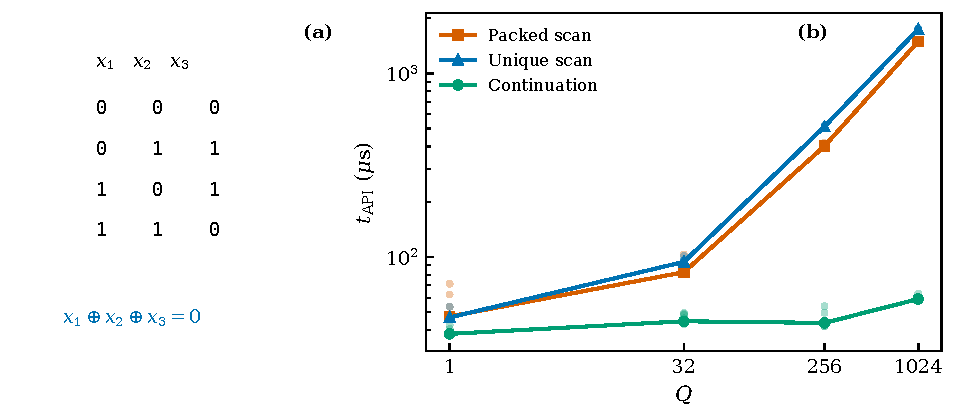
\includegraphics[width=\linewidth]{figures/portable-run-b69220b3a27348ad.result/dd-memory-parity.pdf}
\caption{Retain the relation rather than its list of instances. (a) In the uniform three-bit even-parity law, each pair is independent but two bits determine the third. A running parity state represents the allowed continuations. (b) Archived timings for the 19-bit law with 262,144 distinct worlds, queries fixing four prefix coordinates and batch size $Q$. All displayed prefix queries have count 16,384. The plotted $t_{\rm API}$ is warm full-API time per batch. Dots are all eleven samples and lines join medians. Build, query preparation and first-process compilation are excluded. The campaign also records capacity refusals and a duplicate-heavy control in which direct scan wins.}
\label{fig:dd-memory-parity}
\end{figure}

\subsection{What the language comparisons establish}
The language campaigns test a longer chain: extracting source descriptions, choosing evidence and composing an answer with a language model. Their controls keep those stages distinguishable. In the news experiment, 609 articles supply a 48-question held-out MultiHop slice. At a 2,000-token evidence budget, Parallax answers 40 questions correctly, flat retrieval 39 and the RAPTOR implementation 35. The comparison called the \emph{metadata control} also answers 40. This is a deliberately simpler readout of the same ingested collection: it uses the same original passages, frozen passage embeddings, source identities and publication dates. The same query compiler separates the question into facets and applies any explicit source/date constraints. It then scores every passage directly by the query--passage inner product, selects up to twenty candidates per facet, and uses the common 2,000-token context packing and reader. It bypasses the semantic cards and the hierarchical representation. Thus the control measures what the shared ingestion and flat, condition-aware retrieval already achieve. The comparison holds Atlas's shared ingestion and conditional retrieval stages fixed. All 48 resulting contexts are byte-identical to Parallax's. For this query family the corrected method successfully preserves the same fine-passage target, while the accuracy result leaves the value of its different internal execution to be assessed through cost and scaling.

The QASPER scientific-paper question-answering test covers 256 questions, of which 235 have positive evidence. At a 4,000-token budget, memory and dense retrieval both cover 182 of those 235 questions, compared with 179 for hybrid and 171 for lexical retrieval. Memory and dense retrieval return identical contexts for 252 of the 256 questions. Here the memory route largely reproduces the dense baseline. These are evidence-coverage counts, distinct from the accuracy of the reader's final answer.

LongMem provides a sharper test of relations across a conversational history. With the same reader and a 4,000-token evidence budget, the memory implementation trails dense and hybrid retrieval both in evidence coverage and in final answers. Figure~\ref{fig:dd-memory-reader-controls} shows the answer counts for all 48 questions and the nine-question temporal subset. The weakness falls on precisely the relations and ordering questions that motivate a richer retained representation.
\begin{figure}[htbp]
\centering
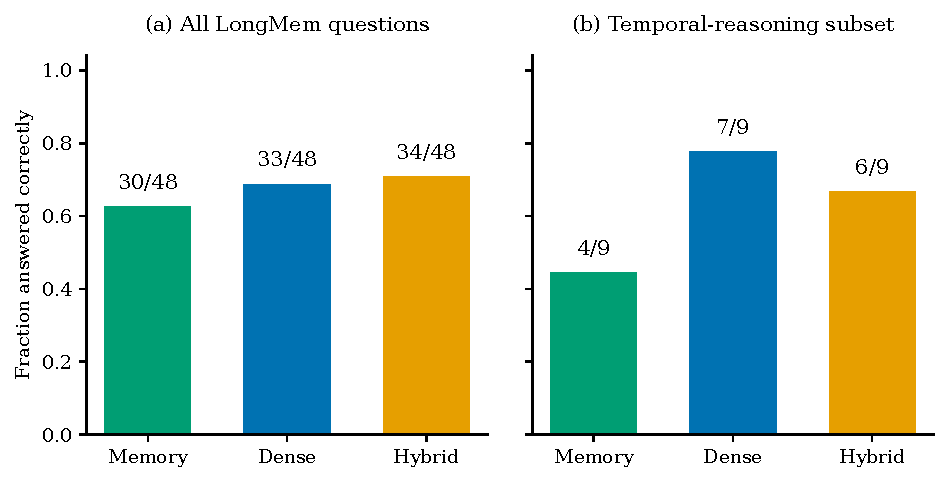
\includegraphics[width=\linewidth]{figures/completion-run-7bd75062068b432b.result/dd-memory-reader-controls.pdf}
\caption{Where the language-memory implementation needs improvement. Archived LongMem answer counts with the same reader and a 4,000-token evidence budget. Memory, dense and hybrid retrieval answer 30, 33 and 34 of the 48 questions correctly. On the nine temporal questions the counts are 4, 7 and 6. The small temporal subset identifies concrete failures to investigate, rather than estimating a universal performance gap.}
\label{fig:dd-memory-reader-controls}
\end{figure}

\subsection{The missing relation and the missing passage}
A source-level audit separates two mechanisms. One development question asks how many projects a person has led or is currently leading. All four required turns are present among the 505 source records, but whole-question embedding retrieval ranks them 63rd, 111th, 208th and 228th. Combining parent and child queries changes those ranks to 66th, 112th, 207th and 241st. Neither the 2,000- nor the 4,000-token context contains the required evidence. The data exists. What is missing is an effective translation from the question to a join over project identities, leadership roles and time, followed by a count. A parent embedding alone does not supply that operation.

A purchase-order question fails differently. Its two support records rank first and ninth under the whole question, and first and seventeenth after merging. Both enter the 2,000-token context, but a first-fit packing rule admits earlier, larger groups at 4,000 tokens and displaces a needed later record. More nominal space can therefore produce a worse evidence set. This is a packing defect, distinguishable from failure to encode a relation during ingestion.

Doubling the evidence budget in the follow-up improves all three methods and helps memory on multi-session questions. Some contexts nevertheless lose previously selected evidence when the budget grows. The audit therefore identifies two different improvements: represent the missing relations explicitly and make evidence packing preserve useful support as capacity increases.

The next implementation should therefore make the relation-bearing part of ingestion explicit. Source-backed entity identities, aliases, roles, events and temporal qualifiers would give a query something on which to execute a join, count or ordering operation. The test is whether this improves held-out relational answers at a fixed evidence budget, with each answer still traceable to its records. A separate branch-preserving packing test should require that enlarging the budget does not discard already selected support. These proposals turn the audit into tests of relation extraction, query execution and evidence packing.

The exact-coordinate campaign and the language campaign now fit together. The former gives an exact composable construction and a measured advantage over scans on the displayed query family. The latter shows the cost of not yet extracting or accessing the right relation reliably. Together they make memory a practical development target: retain the structure that answers the question, preserve its witnesses, and measure the failures that tell us what to ingest next.

The nearest comparisons already exploit structure. GraphRAG extracts entities and relations with a language model, forms graph communities and writes multilevel community summaries. Queries map over summaries and combine intermediate answers. Its principal evidence concerns global sensemaking over large corpora, including breadth and diversity judged against vector retrieval. It is not merely a cosine index. What it does not supply is the particular operator-intertwining residual and task-error contract in Eqs.~\eqref{eq:memory-object}--\eqref{eq:memory-task-error}. Whether that additional contract helps depends on a task for which it can be evaluated.\footnote{D. Edge et al., \emph{From Local to Global: A GraphRAG Approach to Query-Focused Summarization}, \href{https://arxiv.org/abs/2404.16130}{arXiv:2404.16130}, version 2.}~\cite{Edge202448436b}

RAPTOR recursively embeds, clusters and summarises text, retaining original chunks alongside higher-level descriptions. Its main evaluated retrieval method searches across all levels rather than relying on a logarithmic tree descent. Its results therefore support the value of multiscale representational content, not an automatic routing complexity advantage. The relevant comparison keeps the reader, context budget and evaluator fixed.~\cite{Sarthi2024a1f229}

Retrieval-Centric Deep Learning in Growing Nonparametric Neural Networks~\cite{Reference2026d462c2} supplies another useful comparison. For a linear layer trained by gradient descent,
\[
 W_T=W_0+\sum_{t=1}^T v_tx_t^T,\qquad
 W_Tq=W_0q+\sum_{t=1}^T v_t(x_t^Tq).
\]
Here $W_0$ is the initial weight matrix, $x_t$ the input at update $t$, $v_t$ the negative learning-rate-scaled gradient with respect to the layer output, and $q$ a new input. The stored weight change and the retained input--update pairs give exactly the same linear prediction. The second performs attention-like retrieval over a training history. Kernel constructions extend the connection by evaluating feature inner products without explicitly constructing all feature coordinates. The retained history can still grow with training. The duality reveals an alternative computation, while compression asks which part of that history the future task actually needs.

The useful application is not restricted to conversational recall. Repeated relational enquiries, exception-sensitive corpus inspection and local predictive models all need a representation that preserves more than an average embedding. A memory system becomes more valuable when its answer includes a route back to the source and a meaningful account of what its compression could have missed.


\section{A result that can be inspected and changed}
\label{section:the-backend-objects-authority-and-revision}

A memory answer needs a route back to its sources. A research result needs that route too, together with a record of the assumptions, calculations and judgements that make it usable. Someone else must be able to inspect it, change its inputs and understand what must be reconsidered. The Writing App is an integrated research environment built around that continuity. It keeps the material, the claims made about it, the work performed on it and the decisions that accept it connected. The manuscript is one view of that research state. Calculations, source passages and review are other views, with tools for moving between them.

Take the gap-aware quantum example. A calculation reports that a gap-aware enlargement sharply reduces the energy error in a specified model and candidate pool. A claim states what that comparison supports. A figure displays it, and a paragraph explains why the energy denominator helped. A reviewer may ask whether the same selection rule works on another Hamiltonian. That question needs the model, pool, selection rule and original result, together with a way to add the next calculation without losing the first.

\subsection{An object carries its grounds}
The system gives each of these objects an identity and an interface. Its detailed material may be a mathematical statement, a table, code, a source passage or a reference to a larger file. Around that material sit a readable summary, typed relationships, revision information and the operations currently allowed. We call this organising pattern a \emph{conceptric envelope}: a unit of knowledge that carries enough context to be inspected and safely used elsewhere.

Figure~\ref{fig:dd-conceptric-envelope} follows the claim in the quantum example. Its exterior says what the result concerns and how to inspect it. Inside are the statement, assumptions and exact grounds. The relationships say that a source supports a method, a calculation tests a configuration, and a figure or paragraph uses the resulting claim. Giving these relationships types makes a practical difference. A source citation supplies documentary support, while a logical premise supplies something the argument requires. A chapter contains a paragraph, while a review task depends on the version it inspected.

Two kinds of digest help here. A readable digest tells another reader or task what the object means. A content digest or revision identifies which version was used. The first makes a large collection navigable, while the second makes a later comparison exact. The app exposes these through the existing claim, source, result and Work interfaces, with each kind of object retaining the details appropriate to its job.

\begin{figure}[htbp]
\centering
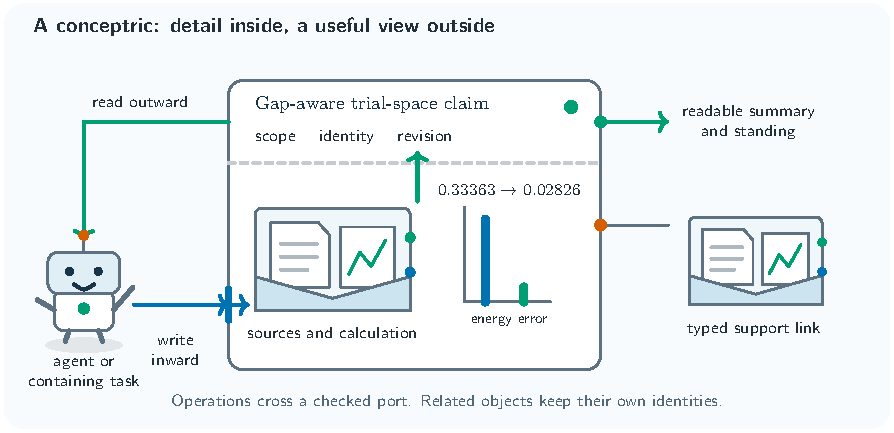
\includegraphics[width=\linewidth]{figures/robot-run-c4d4b3872a904ec0.result/dd-conceptric-envelope.pdf}
\caption{A claim with a readable exterior. The gap-aware comparison retains its model, candidate pool and source/result links, while the containing task receives a concise account of what it can use. The action interface admits changes against the current version. Blue marks the object and its operations, teal the outward flow of observations.}
\label{fig:dd-conceptric-envelope}
\end{figure}

The direction of information is important. Here \emph{inside} means an object's detailed material and local state, and \emph{outside} means its interface and the task that contains or uses it. \emph{Reading goes in to out}: observations of the inner material become the summary or selected detail exposed to that task. A request to open a source points inward, but the information returned from it flows outward. \emph{Writing goes out to in}: an outer intention, such as revising the energy claim, is narrowed to an allowed operation on a particular inner object. Its outcome then becomes visible outside again.

This arrangement gives a task control over its level of detail. A comparison of methods may need a result summary and its conditions. Checking one number may need the precise configuration and table row. Editing a caption needs the figure's data and the current words. The system supplies bounded observations for those different purposes and provides explicit routes to further detail. Semantic selection still matters: the author or agent must ask for the material the inference needs.

\subsection{An authorised change}
The \emph{harness} is the software around the model that prepares its context, exposes tools and routes their requests. It starts with the selected project, the author's question, the relevant objects and the session's role. A working author session and an independent reviewer have different available operations. A child calculation also has a declared task and a place to return its result. These boundaries make responsibility visible before an action is taken.

Suppose the AI wants to link the new calculation to the energy claim. It submits a structured request identifying both objects and the revisions it has inspected. The gateway checks the operation, the role and the project scope. The request then reaches the \emph{owner}, the application component responsible for that kind of change. The owner checks the relevant current identities and records the admitted transition. Source editing adds its own checks on the selected manuscript, exact original passage and proposed replacement. Figure~\ref{fig:dd-ai-tool-harness} shows this route.

\begin{figure}[htbp]
\centering
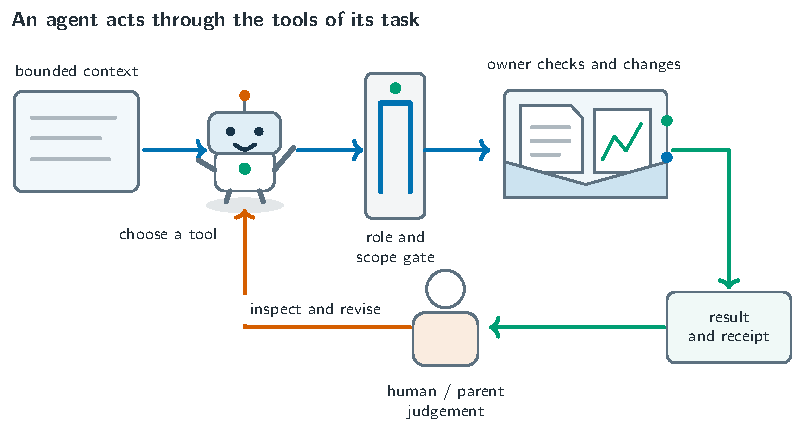
\includegraphics[width=\linewidth]{figures/robot-run-c4d4b3872a904ec0.result/dd-ai-tool-harness.pdf}
\caption{From a model request to an inspectable result. The harness supplies task context and checks permission. The owning operation checks the current basis and records the change. The human and parent task can inspect the same outcome, judge its interpretation and request a revision. The loop keeps the proposal, action and acceptance connected.}
\label{fig:dd-ai-tool-harness}
\end{figure}

The return explains what happened and where to inspect it. For a numerical producer, that includes its inputs, execution outcome and output. For a source change, it includes the affected passage and recorded revision. If a write lands but a later recording step is interrupted, the recovery mechanism is designed to use the retained source effect to distinguish a committed edit from a pending record. It can then finish the record without replaying the source edit.\footnote{The linked implementation account identifies source-inspected recovery branches. The successful figure application described below is not an interrupted-operation test. This account does not display an executed recovery trace.}

Scientific acceptance enters at a different point in the same route. A human or designated model reviewer judges whether the evidence supports the stated interpretation. The literature tool records that judgement alongside the observed passage and the claim version. Numerical checks test a declared calculation. Formal checks test an encoded proposition and its assumptions. The parent task brings those contributions together and records what it accepts. Each participant can inspect the basis of the decision and challenge the relevant step.

The implementation keeps a passage observation separate from the judgement that it supports a claim. A current file identifies the material used. A support judgement says what someone concluded from it. A containing task's acceptance records which contribution it admitted. None substitutes for the others.

\subsection{What the change affects}
Now change the candidate pool used by the quantum calculation. The original result still describes its original pool. The new input gives the next calculation a different basis, and any explanation that intends to use the new result needs attention. A paragraph's wording may remain byte-for-byte unchanged while its supporting comparison has moved. This is why the system tracks a content revision separately from the currentness of its grounds.

Work records make the consequence actionable. A task stores its objective, current standing, declared prerequisites and completion evidence. Acceptance retains the exact prerequisite completions and evidence it consumed. When one of those changes, the current observation can mark that acceptance stale and identify the affected input. A new run, revised interpretation or fresh review can then restore the local chain. The scope of this propagation is the declared dependency graph. It gives the system a precise way to ask what needs reconsidering, while people and reviewers decide how the scientific account should change.

The human interface exposes the same state through manuscript, research, reference, logical-structure and Work views. The AI enters through tools that reach the same owners. A reader can open the claim, follow its result or source, inspect the proposed change and see its outcome. For repository inspection, \nolinkurl{docs/writing-source-map.md} is the entry point, with the transaction in \nolinkurl{src/laplace/manuscript/source_application.py}, context admission in \nolinkurl{src/laplace/writing/turn_admission.py}, and task acceptance in \nolinkurl{src/laplace/work/project_work.py}.

The hierarchy figure in this account followed that route. A supervised calculation produced the stability curves and checked their boundary against the linearised dynamics. We interpreted the result, bound it to the feedback claim, and revised the explanation and figure placement against the current source. The editor preserved the preceding text, recorded the application and rebuilt the PDF. A reader can consequently move from the displayed boundary back to the model and calculation, or forward from the claim to the passage that uses it.

The open-systems discussion gives a useful design comparison. A scientific object's meaning depends on its context: a Hamiltonian convention, candidate pool or source version can change what its conclusion supports. Eigen retains those consequential relationships at the object's boundary, while exposing only the detail needed by the current task. When a surrounding assumption changes, the relevant consumer must be reconsidered. The boundary retains the dependencies that make a local operation safe to compose with the rest of the work.

The connection to the earlier theory is now concrete. A useful representation keeps the distinctions required by an operation and exposes the cost of losing them. For this software, those distinctions include the material, its interpretation, the authority to change it and the evidence on which a decision rests. Preserving them lets a small local operation participate in a larger research process. The same boundary can then be repeated at the level of a calculation, a manuscript section or an entire project.

\section{Research that corrects its interpretation}
\label{section:research-that-can-inspect-its-own-results}

These mechanisms matter most when a result needs to be questioned rather than merely stored. Eigen's campaign on the SuperARC benchmark followed that path: an attractive score prompted closer examination of what the score measured. Its strongest scientific product was the resulting correction.

The original benchmark starts from an algorithmic-information idea: a compact executable account of data can express structure that literal reproduction does not. A program has consequences. It can be run, compared with a target and challenged on new inputs. SuperARC turns that motivation into several finite tests, including sequence reconstruction and prediction. Those are distinct tasks: reproducing a supplied finite prefix does not establish its unseen continuation.\footnote{Hern\'andez-Espinosa et al., \emph{SuperARC: a test for artificial superintelligence based on compressed modelling, recursive prediction and problem complexity}, Nature Communications 17,4885 (2026), \href{https://doi.org/10.1038/s41467-026-73289-5}{doi:10.1038/s41467-026-73289-5}.}~\cite{HernndezEspinosa2026c672f1}

For its reconstruction score, correct answers are divided into non-print/non-ordinal, ordinal and print categories. If their fractions are $\rho_1,\rho_2,\rho_3$, the score is
\begin{equation}
 \phi=\rho_1\delta_1+0.1\rho_2\delta_2+0.01\rho_3\delta_3.
 \label{eq:superarc-score}
\end{equation}
Within each category, $\delta_k$ is a harmonic mean of $\tanh[\mathrm{nBDM}(\mathrm{target})/\mathrm{nBDM}(\mathrm{answer})]$. Normalised block decomposition complexity, nBDM, is a finite operational approximation inspired by algorithmic information theory. The category weights build a preference for generative-looking answers into the instrument. Changing an answer's category can change its contribution by a factor of ten or a hundred without changing execution correctness.

The Eigen SuperARC campaign  generated answers to 100 twelve-term binary sequences using a bare arm, an iterative loop and an execute/fix comparison arm. All three recorded correct outcomes on every target under their respective checking routes. Their answer forms differed sharply: the bare arm mostly printed the sequence, while the two active arms mostly produced generative-looking expressions. Figure~\ref{fig:dd-superarc-controls} shows how those categories and the subsequent format controls affect the score.
\begin{figure}[htbp]
\centering
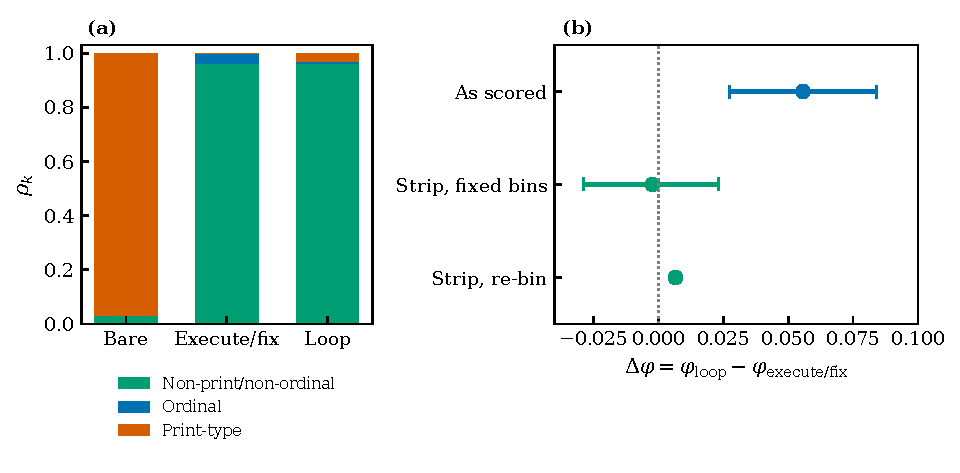
\includegraphics[width=\linewidth]{figures/portable-run-b69220b3a27348ad.result/dd-superarc-controls.pdf}
\caption{The recorded Eigen campaign on the SuperARC reconstruction task. (a) Fractions $\rho_k$ in each correct-answer category for $N=100$ twelve-term binary targets. All arms recorded correct outcomes through their distinct checking routes. (b) Loop-minus-execute/fix score difference $\Delta\phi$. Stripping commentary with categories fixed removes the positive separation. Bars are the archived 95\% paired-bootstrap intervals at resample size 100, seed 20260804 and 100 resamples. No interval was reported for the re-binned point. Formula-text scoring, program correctness and unequal search protocols prevent a causal recursion claim.}
\label{fig:dd-superarc-controls}
\end{figure}

The actual scored object requires care. Complexity was computed from formula text, not simply from the executable program retained beside it. Bare-arm correctness used scorer-side translation. The other arms used their banked programs, with an additional translation cross-check that did not always agree or succeed. This distinction matters because the scoring representation and the executable witness can otherwise appear to be the same object. The campaign preserved enough of both to expose the mismatch.

The adversarial follow-up found a direct confound. Commentary was much more common in loop answers, and the normalised text-complexity calculation could reward that extra text without adding generative information. Stripping commentary while holding answer categories fixed removes the positive loop-minus-execute/fix separation, as Figure~\ref{fig:dd-superarc-controls} shows. Reclassifying the stripped answers is a different protocol and gives a different point estimate. The apparent advantage was therefore sensitive to the representation being scored.

This correction is the campaign's most informative outcome. The system built an instrument, generated and executed candidates, preserved a frozen result, tested competing explanations and revised the interpretation. Unequal prompts and search access still require a controlled follow-up to isolate the effect of execution feedback. The demonstrated capacity is sustained research that leaves its conclusions open to inspection and correction.

The same process can be applied to the system's own explanation. A book describing the present research environment was written and revised using that environment: The Living System Guide . It explains the objects, tools, human decisions and recoverable work described above. Writing it therefore tested whether the system could use its own evidence to make its operation clearer.

One example concerned the effect of changing a source. Several claims used that source, and a further conclusion drew those claims together. The book's diagram needed to distinguish a change in the supporting material from a change in the conclusion's actual wording. Inspection of the implemented behaviour exposed where the explanation blurred those two things, and the caption was corrected. The useful outcome was a clearer account of when a reader should reconsider a conclusion even though its sentence has not changed.

The book also had to work for someone who had not built the system. An independent reader identified passages and figures that were difficult to follow. Those findings led to revisions, a rebuilt book and a focused reread. That cycle connects a technical construction to a usable explanation: the reader's difficulty becomes a concrete revision, whose source and rendered outcome remain inspectable.

A larger theoretical argument tests a different use of the same infrastructure. Foundations of Synthetics , the work from which the retained-state, residual and refinement constructions in this account were drawn, develops its argument through linked derivations, finite examples and explanatory figures. Those pieces retain their claims, evidence and revision history, so they can be extended and inspected separately while the manuscript explains how they fit together. The demonstration is the construction and maintenance of a connected argument, alongside the individual mathematical results it contains.

The three demonstrations now form a progression: investigate a benchmark, improve the system's own explanation, and build a larger theoretical account from inspectable parts. Each leaves material that can support the next piece of work. This is the practical basis of guided self-improvement: an agent helps build and test a capability, while an author sets its direction and acceptance conditions. To make that capacity useful beyond these projects, the same objects and operations must become understandable and extensible to another developer.


\section{From implemented mechanisms to an extensible core}
\label{section:from-a-working-core-to-an-extensible-sdk}

The route from these demonstrations to a reusable product is to expose the working core independently of this particular editor. Its organising unit is the object introduced above: an envelope carrying material, meaning and the grounds for using it. Such objects can be nested or linked without losing access to their detail. A result belongs to a calculation task, that task contributes to a comparison, and the comparison contributes to the project. Each level can expose a concise account while retaining a route to its detailed grounds. The \emph{altitude of a task} is the level at which its decision is being made: choosing a research direction, checking a calculation and editing a sentence need different observations of the same underlying work.

Figure~\ref{fig:dd-nested-work-sdk} follows this pattern through a parent task, a worker and an independent reviewer. The parent asks a bounded question and supplies the relevant context. The worker reads the necessary sources or runs the declared calculation, then returns a contribution with its evidence. The reviewer inspects that exact contribution. The parent consumes both the result and the review before deciding what belongs in the larger account. Context descends with the question, while observations and findings return with a known scope.

The current Work mechanism already distinguishes nesting from dependence. A containing goal contributes to the scope of its child tasks. A prerequisite relation specifies which completed contribution a later task relies on. Changing the parent goal can therefore change a child's scope, while changing an accepted prerequisite can require a consumer's acceptance to be reconsidered. This gives composed work an explicit basis at each level instead of treating the word \emph{done} as a timeless property. Historical completions remain recorded, while missing evidence about what they depended on remains visible.

\begin{figure}[htbp]
\centering
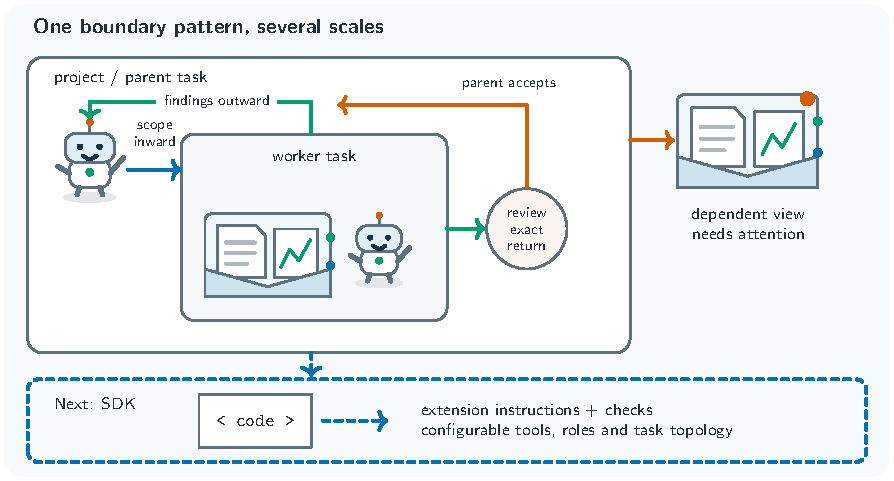
\includegraphics[width=\linewidth]{figures/robot-run-c4d4b3872a904ec0.result/dd-nested-work-sdk.pdf}
\caption{Composition across task altitudes. The parent sends a scoped question to a worker, receives an evidence-bearing contribution and consumes independent findings. Source, result and claim remain addressable within the child task. The amber marker on the neighbouring object shows where a changed input creates local review work. The dashed panel identifies the next SDK capabilities, using the same object and boundary vocabulary.}
\label{fig:dd-nested-work-sdk}
\end{figure}

Tools compose through the same discipline. One operation returns an identified result and the exact routes for inspecting or using it. The next operation consumes that result under its own conditions. A figure renderer, a claim-binding operation and a manuscript editor can therefore cooperate without sharing a hidden conversational memory. Their interfaces preserve the identity and meaning needed at the join.

The present system supplies the specialised objects, guarded tools, parent/worker/reviewer roles, bounded context and recorded acceptance used in this account. The next step is to package that working pattern as a standalone SDK. Its object templates should describe their states, allowed transitions, dependency effects and checks. Its extension instructions should travel with the code, so a developer can discover how a new capability fits rather than reconstructing the author's history.

A small extension makes the requirement tangible. An analysis module should declare its input types and revisions, output format, resource limits and failure behaviour. A result it produces should expose its interpretation and limitations, bind to the relevant claim and say which consumers need attention when an input changes. A new client should be able to inspect that result, propose a change and recover an interrupted operation through the same interfaces as the Writing App. The conformance examples should include successful use, a stale input, a repeated request and an attempted change outside the caller's authority.

This leads towards an operating environment for structured knowledge and agent work. An editor presents paragraphs and figures. A laboratory client presents samples and measurements. A research agent receives the objects needed for its task. A future frontend can let the author configure the topology and roles of a session network: which tasks run independently, which wait for evidence, who reviews them and where acceptance returns. The underlying contracts give those different interfaces a common meaning of identity, state and completion.

Source code already has a scoped place in this structure. The implementation exposes declared source inputs and human-granted development operations tied to a checkout, exact basis, permitted paths and checks. Retained source facts and their publication have separate owners. This is narrower than an autonomous ability to rewrite the running system. The SDK should make the relationship discoverable: a module's purpose, dependencies and checks should identify which behaviour a proposed change affects and which review may admit it. A useful increment can then increase the capacity available to build and inspect the next one without losing the boundary of the original permission.

The recursion matters because the same questions recur at each scale. What does this object retain? Which operation may change it? What does the change affect? What evidence makes the result usable? The SDK should make those questions answerable from its own interfaces and examples. A clean-environment test with an unfamiliar developer - one new result type, one second client, one interrupted operation recovered - would show whether the pattern has become a product that other people can extend.

\section{Where the construction earns its cost}
\label{section:the-collection-and-the-next-tests}

The constructions now fit together around a practical question: which distinctions must a description preserve to do its job? The shared-register calculation prices a new distinction. The retained-state and memory constructions show how to carry its dynamical consequences. Loss geometry and spectral analysis reveal which corrections remain accessible. Mean force shows how a subsystem can retain environmental influence after its surroundings are removed from the explicit description. The conditional-displacement result goes further: it absorbs bath coupling exactly, predicts the ground energy and local state with a controlled correction, and reconstructs the conditional bath and the observables in another reference. The quantum and memory prototypes turn these ideas into procedures, while the Writing App keeps their claims, sources and consequences available for further work.

The common method is constructive. Choose the task, retain a representation that supports it, measure the failure under the intended operation and use that failure to decide what to add or change. The examples make the choice tangible: an omitted direction can be worth more than a larger residual, a small internal contrast can preserve a useful query, and an extra register can remove a conflict that further optimisation cannot resolve. The backend applies the same discipline to research objects by retaining the assumptions and evidence needed to use them elsewhere.

The most useful next evaluations are bounded comparisons with clear costs. The quickest engineering test is an unfamiliar developer adding one result type and a second client from the SDK's exported instructions, then recovering an interrupted change. That tests whether the present core has become a capability others can extend. For quantum trial-space growth, compare raw overlap, amplitude-over-gap and estimated energy-gain selection on Hamiltonians not constructed to favour one ranking, using the same candidate pool, preparation access and measurement budget. Include a classical preconditioned subspace baseline where the same matrix access is available, and near-degenerate cases where a denominator becomes unreliable. Keep descent of a Ritz value separate from certification of the global ground state. For spectral filtering, count filter bias, quadrature error, overlap support and finite-shot ratio uncertainty at the requested resolution.

Dynamic Memory needs the corresponding task-aligned comparison. The query propagator should be checked against exact source reconstruction, and incremental updates against full rebuilding, with parsing, affected dependency cones and witness output counted. A small exact fixture cannot establish large-corpus update scaling. Use withheld joint and exception queries alongside ordinary fact lookup and global summarisation. Compare the actual GraphRAG and RAPTOR procedures, condition-aware flat retrieval, exact indexed alternatives and direct scans with the same reader and context budget. Count ingestion, storage, build cost, cold and warm query time, source recovery and answer quality separately. The existing controls make the next improvements specific: extract relation-bearing information, execute the requested join or ordering operation, and preserve useful evidence when the context budget grows.

The judgement of support also needs a test. Independently adjudicated cases should include genuine support, contradiction, a missing premise and a changed source. Measure false acceptance, false rejection, disagreement and review cost, then alter the evidence and check that the recorded judgement is reopened on the correct basis. Together with stale-client and interrupted-operation tests, this evaluates both the quality of a decision and the system's ability to retain what that decision depended on.

The physical calculation now gives this programme a particularly useful test case. At a fixed bath gap, the analytical ground-state prediction and independent numerical comparison are in hand. Extending that control towards a gapless bath requires retaining the very low-frequency part of the spectrum and specifying how cooling, adding bath modes and removing a small symmetry-selecting bias are taken. The separate continuum approximation already identifies where further terms matter: when extrapolated to a bath with much more low-frequency weight, it misses the numerical phase boundary. The refinement residue and contextuality constructions likewise require explicit common-space, composition and measurement assumptions to become one physical reconstruction. These are specific next calculations, building on results that already turn representation into a predictive procedure.

Eigen is worth evaluating as a theory-guided method of construction, backed by working prototypes and an implemented research environment. Some expensive distinctions are unnecessary, while some small omitted distinctions are decisive. The proposed advantage is a system designed to find out which is which, preserve the resulting knowledge and use it in the next construction. An extensible SDK is the practical next step: carry those objects and operations into other tools, make their extension contracts intelligible, and test where the method earns its cost.

\begingroup
\small
\bibliographystyle{plain}
\bibliography{refs}
\endgroup
\end{document}
